%
% A header that lets you compile a chapter by itself, or inside a larger document.
% Adapted from http://stackoverflow.com/questions/3655454/conditional-import-in-latex
%
%
%Use \inbpdocument and \outbpdocument in your individual files, in place of \begin{document} and \end{document}. In your main file, put in a \def \ismaindoc {} before including or importing anything.
%
% David Duvenaud
% June 2011
% 
% ======================================
%
%


\ifx\ismaindoc\undefined
	\newcommand{\inbpdocument}{
		\def \ismaindoc {}
		% Use this header if we are compiling by ourselves.
		\documentclass[a4paper,11pt,authoryear,index]{common/PhDThesisPSnPDF}
		
%\usepackage{draftwatermark}
%\SetWatermarkLightness{0.95}

% ******************************************************************************
% ****************************** Custom Margin *********************************

% Add `custommargin' in the document class options to use this section
% Set {innerside margin / outerside margin / topmargin / bottom margin}  and
% other page dimensions

\ifsetMargin
\else
    \RequirePackage[left=37mm,right=30mm,top=35mm,bottom=30mm]{geometry}
    \setFancyHdr % To apply fancy header after geometry package is loaded
\fi


%\chead{Unfinished draft}
%\cfoot{\texttt{Unfinished draft - compiled on \today{} at \currenttime}}

% *****************************************************************************
% ******************* Fonts (like different typewriter fonts etc.)*************

% Add `customfont' in the document class option to use this section

\ifsetFont
\else
    % Set your custom font here and use `customfont' in options. Leave empty to
    % load computer modern font (default LaTeX font).  

    \RequirePackage{libertine} 
\fi

% *****************************************************************************
% *************************** Bibliography  and References ********************

%\usepackage{cleveref} %Referencing without need to explicitly state fig /table

% Add `custombib' in the document class option to use this section
\ifsetBib % True, Bibliography option is chosen in class options
\else % If custom bibliography style chosen then load bibstyle here

   \RequirePackage[square, sort, numbers, authoryear]{natbib} % CustomBib

% If you would like to use biblatex for your reference management, as opposed to the default `natbibpackage` pass the option `custombib` in the document class. Comment out the previous line to make sure you don't load the natbib package. Uncomment the following lines and specify the location of references.bib file

% \RequirePackage[backend=biber, style=numeric-comp, citestyle=numeric, sorting=nty, natbib=true]{biblatex}
% \bibliography{References/references} %Location of references.bib only for biblatex

\fi


% changes the default name `Bibliography` -> `References'
\renewcommand{\bibname}{References}


% *****************************************************************************
% *************** Changing the Visual Style of Chapter Headings ***************
% Uncomment the section below. Requires titlesec package.

%\RequirePackage{titlesec}
%\newcommand{\PreContentTitleFormat}{\titleformat{\chapter}[display]{\scshape\Large}
%{\Large\filleft{\chaptertitlename} \Huge\thechapter}
%{1ex}{}
%[\vspace{1ex}\titlerule]}
%\newcommand{\ContentTitleFormat}{\titleformat{\chapter}[display]{\scshape\huge}
%{\Large\filleft{\chaptertitlename} \Huge\thechapter}{1ex}
%{\titlerule\vspace{1ex}\filright}
%[\vspace{1ex}\titlerule]}
%\newcommand{\PostContentTitleFormat}{\PreContentTitleFormat}
%\PreContentTitleFormat


% *****************************************************************************
% **************************** Custom Packages ********************************
% *****************************************************************************


% ************************* Algorithms and Pseudocode **************************

%\usepackage{algpseudocode} 


% ********************Captions and Hyperreferencing / URL **********************

% Captions: This makes captions of figures use a boldfaced small font. 
%\RequirePackage[small,bf]{caption}

\RequirePackage[labelsep=space,tableposition=top]{caption} 
%\renewcommand{\figurename}{Figure} %to support older versions of captions.sty
\captionsetup{belowskip=12pt,aboveskip=4pt}

% ************************ Formatting / Footnote *******************************

%\usepackage[perpage]{footmisc} %Range of footnote options 


% ****************************** Line Numbers **********************************

%\RequirePackage{lineno}
%\linenumbers

% ************************** Graphics and figures *****************************

%\usepackage{rotating}
%\usepackage{wrapfig}
%\usepackage{float}
\usepackage{subfig} %note: subfig must be included after the `caption` package. 


% ********************************* Table **************************************

%\usepackage{longtable}
%\usepackage{multicol}
%\usepackage{multirow}
%\usepackage{tabularx}


% ***************************** Math and SI Units ******************************

\usepackage{amsfonts}
\usepackage{amsmath}
\usepackage{amssymb}
%\usepackage{siunitx} % use this package module for SI units


% ******************************************************************************
% ************************* User Defined Commands ******************************
% ******************************************************************************

% *********** To change the name of Table of Contents / LOF and LOT ************

%\renewcommand{\contentsname}{My Table of Contents}
%\renewcommand{\listfigurename}{List of figures}
%\renewcommand{\listtablename}{List of tables}


% ********************** TOC depth and numbering depth *************************

\setcounter{secnumdepth}{2}
\setcounter{tocdepth}{2}

% ******************************* Nomenclature *********************************

% To change the name of the Nomenclature section, uncomment the following line

%\renewcommand{\nomname}{Symbols}


% ********************************* Appendix ***********************************

% The default value of both \appendixtocname and \appendixpagename is `Appendices'. These names can all be changed via: 

%\renewcommand{\appendixtocname}{List of appendices}
%\renewcommand{\appendixname}{Appndx}

		% All my custom preamble stuff.  Shouldn't overlap with anything in official-preamble


% Paths to figure and table directories.
\newcommand{\symmetryfigsdir}{figures/symmetries}
\newcommand{\topologyfiguresdir}{figures/topology}
\newcommand{\infinitefiguresdir}{figures/infinite}
\newcommand{\grammarfiguresdir}{figures/grammar}
\newcommand{\introfigsdir}{figures/intro}
\newcommand{\gplvmfiguresdir}{figures/gplvm}
\newcommand{\warpedfiguresdir}{figures/warped-mixtures}
\newcommand{\deeplimitsfiguresdir}{figures/deep-limits}
\newcommand{\quadraturefigsdir}{figures/quadrature}
\newcommand{\additivefigsdir}{figures/additive}
\newcommand{\decompfigsdir}{figures/decomp}
\newcommand{\examplefigsdir}{figures/worked-example}


\usepackage{bm}  % for warped mixtures - is this necessary?
\usepackage{booktabs}
\usepackage{tabularx}
\usepackage{multirow}
\usepackage{datetime}
\renewcommand{\tabularxcolumn}[1]{>{\arraybackslash}m{#1}}
\usepackage{relsize}
\usepackage{graphicx}
\usepackage{amsmath,amssymb,textcomp}
\usepackage{nicefrac}
\usepackage{amsthm}
\usepackage{tikz}
\usetikzlibrary{arrows}
\usetikzlibrary{calc}
\usepackage{nth}
\usepackage{rotating}
\usepackage{array}
\usepackage{fp}
\usepackage[hyperpageref]{backref}
\def\foo{\hspace{\fill}\mbox{}\linebreak[0]\hspace*{\fill}}
\renewcommand*{\backref}[1]{}
\renewcommand*{\backrefalt}[4]{%
\ifcase #1 %
%
\or
\foo(page #2)%
\else
\foo(pages #2)%
\fi
}

\usepackage{cleveref}
\crefname{equation}{equation}{equations}


%% For submission, make all render blank.
%%%%%%%%%%%%%%%%%%%%%%%%%%%%%%%%%%%%%%%%%%%%%%%%%%%%%%%%%%
%%%% EDITING HELPER FUNCTIONS  %%%%%%%%%%%%%%%%%%%%%%%%%%%
%%%%%%%%%%%%%%%%%%%%%%%%%%%%%%%%%%%%%%%%%%%%%%%%%%%%%%%%%%

%% NA: needs attention (rough writing whose correctness needs to be verified)
%% TBD: instructions for how to fix a gap ("Describe the propagation by ...")
%% PROBLEM: bug or missing crucial bit 

%% use \fXXX versions of these macros to put additional explanation into a footnote.  
%% The idea is that we don't want to interrupt the flow of the paper or make it 
%% impossible to read because there are a bunch of comments.

%% NA's (and TBDs, those less crucially) should be written so 
%% that they flow with the text.

\definecolor{WowColor}{rgb}{.75,0,.75}
\definecolor{SubtleColor}{rgb}{0,0,.50}

% inline
\newcommand{\NA}[1]{\textcolor{SubtleColor}{ {\tiny \bf ($\star$)} #1}}
\newcommand{\LATER}[1]{\textcolor{SubtleColor}{ {\tiny \bf ($\dagger$)} #1}}
\newcommand{\TBD}[1]{\textcolor{SubtleColor}{ {\tiny \bf (!)} #1}}
\newcommand{\PROBLEM}[1]{\textcolor{WowColor}{ {\bf (!!)} {\bf #1}}}

% as margin notes

\newcounter{margincounter}
\newcommand{\displaycounter}{{\arabic{margincounter}}}
\newcommand{\incdisplaycounter}{{\stepcounter{margincounter}\arabic{margincounter}}}

\newcommand{\fTBD}[1]{\textcolor{SubtleColor}{$\,^{(\incdisplaycounter)}$}\marginpar{\tiny\textcolor{SubtleColor}{ {\tiny $(\displaycounter)$} #1}}}

\newcommand{\fPROBLEM}[1]{\textcolor{WowColor}{$\,^{((\incdisplaycounter))}$}\marginpar{\tiny\textcolor{WowColor}{ {\bf $\mathbf{((\displaycounter))}$} {\bf #1}}}}

\newcommand{\fLATER}[1]{\textcolor{SubtleColor}{$\,^{(\incdisplaycounter\dagger)}$}\marginpar{\tiny\textcolor{SubtleColor}{ {\tiny $(\displaycounter\dagger)$} #1}}}

%\renewcommand{\LATER}[1]{}
%\renewcommand{\fLATER}[1]{}
%\renewcommand{\TBD}[1]{}
%\renewcommand{\fTBD}[1]{}
%\renewcommand{\PROBLEM}[1]{}
%\renewcommand{\fPROBLEM}[1]{}
%\renewcommand{\NA}[1]{}


% HUMBLE WORDS: shown slightly smaller when in normal text
% Thanks to Christian Steinruecken!

% HUMBLE WORDS: shown slightly smaller when in normal text
%
\makeatletter%
%\def\@humbleformat#1{{\fontsize{}{1em}\selectfont #1}}
%\def\@humbleformat#1{\textsmaller{#1}}%
\newlength{\nonHumbleHeight}
\def\@humbleformat#1{{\settoheight{\nonHumbleHeight}{#1}\resizebox{!}{0.94\nonHumbleHeight}{#1}}}%
\def\@idxhumbleformat#1{{\relscale{0.95}{#1}}}%
%\def\@humbleformat#1{{#1}}%
\def\declareHumble#1#2{%
  \expandafter\def\csname #1\endcsname{\@humbleformat{#2}}%
  \expandafter\def\csname s#1\endcsname{{#2}}%
  \expandafter\def\csname idx#1\endcsname{{\@idxhumbleformat{#2}}}%
}%
\def\humble#1{\@humbleformat{#1}}%
\def\idxhumble#1{\@idxhumbleformat{#1}}%
\makeatother%

% Convenient indexing for humble abbreviations
\def\humbleindex#1#2{\index{#1@\idxhumble{#1}}}



% TODO: Clean up duplicates
\declareHumble{ANOVA}{ANOVA}
\declareHumble{ARD}{ARD}
\declareHumble{BIC}{BIC}
\declareHumble{BMC}{BMC}
\declareHumble{bq}{BQ}
\declareHumble{CRP}{CRP}
\declareHumble{dirpro}{DP}
\declareHumble{HDMR}{HDMR}
\declareHumble{GAM}{GAM}
\declareHumble{GEM}{GEM}
\declareHumble{GMM}{GMM}
\declareHumble{gplvm}{GP-LVM}
\declareHumble{gpml}{GPML}
\declareHumble{GPML}{GPML}
\declareHumble{gprn}{GPRN}
\declareHumble{gpt}{GP}
\declareHumble{gp}{GP}
\declareHumble{HKL}{HKL}
\declareHumble{HMC}{HMC}
\declareHumble{ibp}{IBP}
\declareHumble{iGMM}{iGMM}
\declareHumble{iwmm}{iWMM}
\declareHumble{kCP}{CP}
\declareHumble{kCW}{CW}
\declareHumble{kC}{C}
\declareHumble{KDE}{KDE}
\declareHumble{kLin}{Lin}
\declareHumble{KPCA}{KPCA}
\declareHumble{kPer}{Per}
\declareHumble{kRQ}{RQ}
\declareHumble{kSE}{SE}
\declareHumble{kWN}{WN}
\declareHumble{Lin}{Lin}
\declareHumble{LBFGS}{L-BFGS}
\declareHumble{mcmc}{MCMC}
\declareHumble{MKL}{MKL}
\declareHumble{MLP}{MLP}
\declareHumble{MSE}{MSE}
\declareHumble{Per}{Per}
\declareHumble{RMSE}{RMSE}
\declareHumble{RQ}{RQ}
\declareHumble{SBQ}{SBQ}
\declareHumble{seard}{SE-ARD}
\declareHumble{sefull}{SE-\textnormal{full}}
\declareHumble{SEGP}{SE-GP}
\declareHumble{SE}{SE}
\declareHumble{SNR}{SNR}
\declareHumble{SSANOVA}{SS-ANOVA}
\declareHumble{SVM}{SVM}

\newcommand{\kSig}{\boldsymbol\sigma}

\def\subexpr{{\cal S}}
\def\baseker{{\cal B}}
\def\numWinners{k}

\def\ie{i.e.\ }
\def\eg{e.g.\ }
\def\etc{etc.\ }
\let\oldemptyset\emptyset
\let\emptyset 0




% Unify notation between neural-net land and GP-land.
\newcommand{\hphi}{h}
\newcommand{\hPhi}{\vh}
\newcommand{\walpha}{w}
\newcommand{\wboldalpha}{\bw}
\newcommand{\wcapalpha}{\vW}
\newcommand{\lengthscale}{w}

\newcommand{\layerindex}{\ell}



\newcommand{\gpdrawbox}[1]{
\setlength\fboxsep{0pt}
\hspace{-0.15in} 
\fbox{
\includegraphics[width=0.464\columnwidth]{\deeplimitsfiguresdir/deep_draws/deep_gp_sample_layer_#1}
}}



\newcommand{\procedurename}{ABCD}
\newcommand{\genText}[1]{{\sf #1}}



\newcommand{\asdf}{$^{\textnormal{th}}$}

\newcommand{\binarysum}{\sum_{\bf{x} \in \{0,1\}^D}}
\newcommand{\expect}{\mathbb{E}}
\newcommand{\expectargs}[2]{\mathbb{E}_{#1} \left[ {#2} \right]}
\newcommand{\var}{\mathbb{V}}
\newcommand{\varianceargs}[2]{\mathbb{V}_{#1} \left[ {#2} \right]}
\newcommand{\cov}{\operatorname{cov}}
\newcommand{\Cov}{\operatorname{Cov}}
\newcommand{\covargs}[2]{\cov \left[ {#1}, {#2} \right]}
\newcommand{\variance}{\mathbb{V}}
\newcommand{\vecop}[1]{\operatorname{vec} \left( {#1} \right)}

\newcommand{\covarianceargs}[2]{\Cov_{#1} \left[ {#2} \right]}
\newcommand{\colvec}[2]{\left[ \begin{array}{c} {#1} \\ {#2} \end{array} \right]}
\newcommand{\tbtmat}[4]{\left[ \begin{array}{cc} {#1} & {#2} \\ {#3} & {#4} \end{array} \right]}

%\newcommand{\covskinny}[2]{\var\!\left(#1\middle\vert#2\right)} 

\newcommand{\acro}[1]{{\humble{#1}}}
%\newcommand{\vect}[1]{\boldsymbol{#1}}
\newcommand{\vect}[1]{{\bf{#1}}}
\newcommand{\mat}[1]{\mathbf{#1}}
\newcommand{\pderiv}[2]{\frac{\partial #1}{\partial #2}}
\newcommand{\npderiv}[2]{\nicefrac{\partial #1}{\partial #2}}

\newcommand{\pha}{^{\phantom{:}}}

\newcommand{\argmin}{\operatornamewithlimits{argmin}}
\newcommand{\argmax}{\operatornamewithlimits{argmax}}

% The following designed for probabilities with long arguments

\newcommand{\Prob}[2]{P\!\left(\,#1\;\middle\vert\;#2\,\right)}
\newcommand{\ProbF}[3]{P\!\left(\,#1\!=\!#2\;\middle\vert\;#3\,\right)}
\newcommand{\p}[2]{p\!\left(#1\middle\vert#2\right)}
\newcommand{\po}[1]{p\!\left(#1\right)}
\newcommand{\pF}[3]{p\!\left(\,#1\!=\!#2\;\middle\vert\;#3\,\right)} 
\newcommand{\mean}[2]{{m}\!\left(#1\middle\vert#2\right)}



\newcommand{\valpha}{\boldsymbol{\alpha}}
\newcommand{\va}{\vect{a}}
\newcommand{\vA}{\vect{A}}
\newcommand{\vB}{\mat{B}}
\newcommand{\vb}{\vect{b}}
\newcommand{\vC}{\mat{C}}
\newcommand{\vc}{\vect{c}}
\newcommand{\vecf}{\boldsymbol{f}}
\newcommand{\vell}{\vect{\ell}}
\newcommand{\vepsilon}{\boldsymbol{\epsilon}}
\newcommand{\veps}{\boldsymbol{\epsilon}}
\newcommand{\ve}{\boldsymbol{\epsilon}}
\newcommand{\vf}{\vecf}
\newcommand{\vg}{\vect{g}}
\newcommand{\vh}{\vect{h}}
\newcommand{\vI}{\mat{I}}
\newcommand{\vK}{\mat{K}}
\newcommand{\vk}{\vect{k}}
\newcommand{\vL}{\mat{L}}
\newcommand{\vl}{\vect{l}}
\newcommand{\vmu}{\boldsymbol{\mu}}
\newcommand{\vone}{\vect{1}}
\newcommand{\vphi}{\boldsymbol{\phi}}
\newcommand{\vpi}{\boldsymbol{\pi}}
\newcommand{\vq}{\vect{q}}
\newcommand{\vR}{\mat{R}}
\newcommand{\vr}{\vect{r}}
\newcommand{\vsigma}{\boldsymbol{\sigma}}
\newcommand{\vSigma}{\mat{\Sigma}}
\newcommand{\vS}{\mat{S}}
\newcommand{\vs}{\vect{s}}
\newcommand{\vtheta}{\boldsymbol{\theta}}
\newcommand{\vu}{\vect{u}}
\newcommand{\vV}{\mat{V}}
\newcommand{\vW}{\mat{W}}
\newcommand{\vw}{\vect{w}}
\newcommand{\vX}{\mat{X}}
\newcommand{\vx}{\vect{x}}
\newcommand{\vY}{\mat{Y}}
\newcommand{\vy}{\vect{y}}
\newcommand{\vzero}{\vect{0}}
\newcommand{\vZ}{\mat{Z}}
\newcommand{\vz}{\vect{z}}


\newcommand{\netweights}{\alpha}
\newcommand{\vnetweights}{\valpha}

\newcommand{\He}{\mathcal{H}}
\newcommand{\normx}[2]{\left\|#1\right\|_{#2}}
\newcommand{\Hnorm}[1]{\normx{#1}{\He}}
\newcommand{\mmd}{{\rm MMD}}


\newcommand{\mf}{\bar{\vf}}

%\newcommand{\mf}{\mu} %{\bar{\ell}}
\newcommand{\lf}{f} % Likelihood function
\newcommand{\st}{_\star}

% from simpler log-bq writeup
\newcommand{\lftwo}{{\log \ell}}
\newcommand{\mftwo}{{\bar \ell}}
\newcommand{\loggp}{{\log\acro{GP}}}%| \bX, \vy )}}
\newcommand{\loggpdist}{{\acro{GP}(\lftwo)}}%| \vX, \vy )}}


\newcommand{\inv}{^{{\mathsmaller{-1}}}}
\newcommand{\tohalf}{^{{\mathsmaller{\nicefrac{1}{2}}}}}

\newcommand{\Normal}{\mathcal{N}}
\newcommand{\N}[3]{\mathcal{N}\!\left(#1 \middle| #2,#3\right)}
\newcommand{\Nt}[2]{\mathcal{N}\!\left(#1,#2\right)}
\newcommand{\NT}[2]{\mathcal{N}\!\left(#1,#2\right)}
\newcommand{\GPdist}[3]{\mathcal{GP}\!\left(#1 \, \middle| \, #2, #3 \right)}
\newcommand{\bN}[3]{\mathcal{N}\big(#1 \middle| #2,#3\big)}
\newcommand{\boldN}[3]{\text{\textbf{\mathcal{N}}}\big(#1;#2,#3\big)}
\newcommand{\ones}[1]{\mat{1}_{#1}}
\newcommand{\eye}[1]{\mat{E}_{#1}}
\newcommand{\tra}{^{\mathsf{T}}}
%\newcommand{\tra}{^{\top}}
%\mathsf{T}
\newcommand{\trace}{\operatorname{tr}}
\newcommand{\shift}{\operatorname{shift}}
\renewcommand{\mod}{\operatorname{mod}}
\newcommand{\deq}{:=}
\newcommand{\oneofk}{\operatorname{one-of-k}}
%\newcommand{\degree}{^\circ}

\newcommand{\GPt}[2]{\mathcal{GP}\!\left(#1,#2\right)}
%\newcommand{\GPt}[2]{\gp\!\left(#1,#2\right)}

\DeclareMathOperator{\tr}{tr}
\DeclareMathOperator{\chol}{chol}
\DeclareMathOperator{\diag}{diag}

\newenvironment{narrow}[2]{%
  \begin{list}{}{%
  \setlength{\topsep}{0pt}%
  \setlength{\leftmargin}{#1}%
  \setlength{\rightmargin}{#2}%
  \setlength{\listparindent}{\parindent}%
  \setlength{\itemindent}{\parindent}%
  \setlength{\parsep}{\parskip}}%
\item[]}{\end{list}}



\newcommand{\dist}{\ \sim\ }
\def\given{\,|\,}

% Table stuff
\newcolumntype{C}[1]{>{\centering\let\newline\\\arraybackslash\hspace{0pt}}m{#1}}
\newcolumntype{L}[1]{>{\raggedright\let\newline\\\arraybackslash\hspace{0pt}}m{#1}}
\newcolumntype{R}[1]{>{\raggedleft\let\newline\\\arraybackslash\hspace{0pt}}m{#1}}


\def\ie{i.e.\ }
\def\eg{e.g.\ }
\def\iid{i.i.d.\ }
%\def\simiid{\sim_{\mbox{\tiny iid}}}
\def\simiid{\overset{\mbox{\tiny iid}}{\sim}}
\def\simind{\overset{\mbox{\tiny \textnormal{ind}}}{\sim}}
\def\eqdist{\stackrel{\mbox{\tiny d}}{=}}
%\newcommand{\distas}[1]{\mathbin{\overset{#1}{\kern \z@ \sim}}}
%TODO: fix this - it worked outside the thesis!
\newcommand{\distas}[1]{\mathbin{\overset{#1}{\sim}}}

\def\Reals{\mathbb{R}}

\def\Uniform{\mbox{\rm Uniform}}
\def\Bernoulli{\mbox{\rm Bernoulli}}
\def\GP{\mathcal{GP}}
\def\GPLVM{\mathcal{GP-LVM}}




% Kernel stuff

\def\iva{\vect{\inputVar}}
\def\ivaone{\inputVar}
\def\inputVar{x}
\def\InputVar{X}
\def\InputSpace{\mathcal{X}}
\def\outputVar{y}
\def\OutputSpace{\mathcal{Y}}
\def\function{f}
\def\kernel{k}
\def\KernelMatrix{K}
\def\SumKernel{\sum}
\def\ProductKernel{\prod}
\def\expression{e}
\def\feat{\vh}

\newcommand{\kerntimes}{ \! \times \!}
\newcommand{\kernplus}{ \, + \,}


% Proof stuff
\theoremstyle{plain}
\newtheorem{theorem}{Theorem}[section]
\newtheorem{lemma}[theorem]{Lemma}
\newtheorem{prop}[theorem]{Proposition}
\newtheorem{proposition}{Proposition}
\newtheorem*{cor}{Corollary}

% For infinite bq
\newcommand{\iv}{\theta}
\newcommand{\viv}{\vtheta}

% For intro chapter
\newcommand{\funcval}{\vf(\vX)}
\newcommand{\testpoint}{{\vx^\star}}

\newcommand{\underwrite}[2]{{\underbrace{#1}_{\textnormal{#2}}}}



% For kernel figures
\newcommand{\fhbig}{2cm}%
\newcommand{\fwbig}{3cm}%
\newcommand{\kernpic}[1]{\includegraphics[height=\fhbig,width=\fwbig]{\grammarfiguresdir/structure_examples/#1}}%
\newcommand{\kernpicr}[1]{\rotatebox{90}{\includegraphics[height=\fwbig,width=\fhbig]{\grammarfiguresdir/structure_examples/#1}}}%
\newcommand{\addkernpic}[1]{{\includegraphics[height=\fhbig,width=\fwbig]{\grammarfiguresdir/additive_multi_d/#1}}}%
\newcommand{\largeplus}{\tabbox{{\Large+}}}%
\newcommand{\largeeq}{\tabbox{{\Large=}}}%
\newcommand{\largetimes}{\tabbox{{\Large$\times$}}}%
\newcommand{\fixedx}{$x$ (with $x' = 1$)}%


		% ************************ Thesis Information & Meta-data **********************

%% The title of the thesis
%\title{Structured Gaussian Process Models} 
%\title{Automatic Model Construction \\ through \\ Structured Gaussian Processes}
%\title{Automatic Model-Building \\ through \\ Structured Gaussian Processes}
%\title{Automatic Modeling \\ with \\ Structured Gaussian Processes}    
\title{Automatic Model Construction \\ with Gaussian Processes}
%\title{Automatic Model Construction}
%\title{Automating Statistical Model Construction}


%\texorpdfstring is used for PDF metadata. Usage:
%\texorpdfstring{LaTeX_Version}{PDF Version (non-latex)} eg.,
%\texorpdfstring{$sigma$}{sigma}

%% The full name of the author
\author{David Kristjanson Duvenaud}

%% Department (eg. Department of Engineering, Maths, Physics)
%\dept{Department of Engineering}

%% University and Crest
\university{University of Cambridge}
\crest{
\includegraphics[width=0.25\textwidth]{University_Crest}}

%% You can redefine the submission text:
% Default as per the University guidelines: This dissertation is submitted for
% the degree of Doctor of Philosophy
%\renewcommand{\submissiontext}{change the default text here if needed}

%% Full title of the Degree 
\degree{Doctor of Philosophy}
 
%% College affiliation (optional)
\college{Pembroke College}

%% Submission date
\degreedate{June 2014} 

%% Meta information
\subject{LaTeX} \keywords{{LaTeX} {PhD Thesis} {Engineering} {University of Cambridge}}



		\begin{document}
	}	
	\newcommand{\outbpdocument}[1]{

		% Fake chapters so references aren't broken
\label{ch:intro}                
\label{ch:kernels}
\label{ch:grammar}
\label{ch:description}
\label{ch:additive}
\label{ch:deeplimits}
\label{ch:discussion}
		%\bibliographystyle{common/CUEDthesis}
		\bibliographystyle{plainnat}
		\bibliography{references.bib}
		\end{document}
	}	
\else
	%If we're inside another document, no need to re-start the document.
	\ifx\inbpdocument\undefined
		\newcommand{\inbpdocument}{}
		\newcommand{\outbpdocument}[1]{}
	\fi
\fi

\inbpdocument



\chapter{Dropout in Gaussian processes}
\label{ch:additive}





\section{Dropout in Gaussian processes}



Dropout is a method for regularizing neural networks \citep{hinton2012improving, srivastava2013improving}.
Training with dropout entails randomly and independently ``dropping'' (setting to zero) some proportion $p$ of features or inputs, in order to improve the robustness of the resulting network by reducing co-dependence between neurons.
To maintain similar overall activation levels, weights are multiplied by $\nicefrac{1}{p}$ at test time. Alternatively, feature activations are multiplied by $\nicefrac{1}{p}$ during training.
At test time, the set of models defined by all possible ways of dropping-out neurons is averaged over, usually in an approximate way.

\citet{baldi2013understanding} and \citet{wang2013fast} analyzed dropout in terms of the effective prior induced by this procedure in several models, such as linear and logistic regression.
In this section, we examine the priors on functions that result from performing dropout in the one-hidden-layer neural network implicitly defined by a \gp{} (equation \eqref{eq:one-layer-nn}).


\subsection{Dropout on feature activations}

First, we examine the prior that results from randomly dropping features from $\hPhi(\vx)$ with probability $p$.
If these features have a weight distribution with finite moments
$\expectargs{}{ \alpha_i} = \mu, \varianceargs{}{\alpha_i} = \sigma^2$,
then the distribution of weights after each one has been dropped out with probability $p$ is:
\begin{align}
r_i \simiid \textnormal{Ber}(p)
\qquad
\expectargs{}{ r_i \alpha_i} = p\mu, \varianceargs{}{r_i \alpha_i} = p^2 \sigma^2 \;.
\end{align}
However, after we increase the remaining activations to maintain the same expected activation by multiplying them by $\nicefrac{1}{p}$, the resulting moments are again:
\begin{align}
\expectargs{}{ \frac{1}{p} r_i \alpha_i } = \frac{p}{p}\mu = \mu, \quad \varianceargs{}{ \frac{1}{p} r_i \alpha_i} = \frac{p^2}{p^2} \sigma^2 = \sigma^2 \;.
\end{align}
%Since only the first two moments of the weight variance matter, the resulting \gp{} remain
Thus, dropping out features of an infinitely-wide MLP does not change the model at all, since no individual feature can have more than infinitesimal contribution to the network output.
%Is there a better way to drop out features that would lead to robustness?

\subsection{Dropping out inputs}

In a \gp{} with kernel ${k(\vx, \vx') = \prod_{d=1}^D k_d(\vx_d, \vx_d')}$, exact averaging over all possible ways of dropping out inputs with probability $\nicefrac{1}{2}$ results in a mixture of \gp{}s, each depending on only a subset of the inputs:
\begin{align}
p \left( f(\vx) \right)= \frac{1}{2^D} \sum_{\vr \in \{0,1\}^D}  \textnormal{\gp} \left(0, \prod_{d=1}^D k_d(\vx_d, \vx_d')^{r_d} \right)
\label{eq:dropout-mixture}
\end{align}
We present two results ways to gain intuition about this model.

First, if the kernel on each dimension has the form ${k_d(\vx_d, \vx_d') = g \left( \frac{\vx_d - \vx_d'}{\lengthscale_d} \right)}$, as does the \humble{SE} kernel \eqref{eq:se_kernel}, then any input dimension can be dropped out by setting its lengthscale $\lengthscale_d$ to $\infty$.
Thus, dropout on the inputs of a \gp{} corresponds to a spike-and-slab prior on lengthscales, with each dimension independently having $w_d = \infty$ with probability $\nicefrac{1}{2}$.



Another way to understand the resulting prior is to note that the dropout mixture \eqref{eq:dropout-mixture} has the same covariance as
\begin{align}
f(\vx) \sim \textnormal{\gp} \left(0, \frac{1}{2^{-2D}} \sum_{\vr \in \{0,1\}^D}  \prod_{d=1}^D k_d(\vx_d, \vx_d')^{r_d} \right)
\label{eq:additive-gps}
\end{align}

A \gp{} whose covariance is a sum of kernels corresponds to a sum of functions, each distributed according to a \gp{}.  Therefore, \eqref{eq:additive-gps} describes a sum of $2^D$ functions, each depending on a different subset of the inputs.
This model class was studied by \citet{duvenaud2011additive11}, who showed that exact inference in these models can be performed in $\mathcal{O}(N^2 D^2 + N^3)$.
%Thus, the dropout prior is closely related to a model which learns many functions, each of which only depends on a subset of the inputs.



In this chapter, we introduce a Gaussian process model of functions which are $\textit additive$.  An additive function is one which decomposes into a sum of low-dimensional functions, each depending on only a subset of the input variables. Additive GPs generalize both Generalized Additive Models, and the standard GP models which use squared-exponential kernels.  Hyperparameter learning in this model can be seen as Bayesian Hierarchical Kernel Learning (HKL).  We introduce an expressive but tractable parameterization of the kernel function, which allows efficient evaluation of all input interaction terms, whose number is exponential in the input dimension.  The additional structure discoverable by this model results in state-of-the-art predictive power in regression tasks, as well as increased interpretability.

\section{Introduction}
%$f: {\bf x} \mapsto y$
Most statistical regression models in use today are of the form: $g(y) = f(x_1) + f(x_2) + \dots + f(x_D)$.  Popular examples include logistic regression, linear regression, and Generalized Linear Models\cite{nelder1972generalized}.  This family of functions, known as Generalized Additive Models (GAM)\cite{hastie1990generalized}, are typically easy to fit and interpret.   Some extensions of this family, such as smoothing-splines ANOVA \cite{wahba1990spline}, add terms depending on more than one variable.  However, such models generally become intractable and difficult to fit as the number of terms increases.

At the other end of the spectrum are kernel-based models, which typically allow the response to depend on all input variables simultaneously.  These have the form: $y = f(x_1, x_2, \dots, x_D)$.  A popular example would be a Gaussian process model using a squared-exponential (or Gaussian) kernel.  We denote this model as SE-GP.  This model is much more flexible than the GAM, but its flexibility makes it difficult to generalize to new combinations of input variables. %To the extent that a set of variables is relevant to the output, this model must be highly uncertain about any novel combination of those variables.

In this paper, we introduce a Gaussian process model that generalizes both GAMs and the SE-GP.  This is achieved through a kernel which allow additive interactions of all orders, ranging from first order interactions (as in a GAM) all the way to $D$th-order interactions (as in a SE-GP).  Although this kernel amounts to a sum over an exponential number of terms, we show how to compute this kernel efficiently, and introduce a parameterization which limits the number of hyperparameters to $O(D)$.  A Gaussian process with this kernel function (an additive GP) constitutes a powerful model that allows one to automatically determine which orders of interaction are important.  We show that this model can significantly improve modeling efficacy, and has major advantages for model interpretability.  This model is also extremely simple to implement, and we provide example code.

We note that a similar breakthrough has recently been made, called Hierarchical Kernel Learning (HKL)\cite{DBLP:journals/corr/abs-0909-0844}.  HKL explores a similar class of models, and sidesteps the possibly exponential number of interaction terms by cleverly selecting only a tractable subset.  However, this method suffers considerably from the fact that cross-validation must be used to set hyperparameters.  In addition, the machinery necessary to train these models is immense.  Finally, on real datasets, HKL is outperformed by the standard SE-GP \cite{DBLP:journals/corr/abs-0909-0844}.

\section{Gaussian Process Models}

Gaussian processes are a flexible and tractable prior over functions, useful for solving regression and classification tasks\cite{rasmussen38gaussian}.  The kind of structure which can be captured by a GP model is mainly determined by its \emph{kernel}: the covariance function.  One of the main difficulties in specifying a Gaussian process model is in choosing a kernel which can represent the structure present in the data.  For small to medium-sized datasets, the kernel has a large impact on modeling efficacy.
  

%\subsection{Additivity in a GP}
\begin{figure}
\centering
\begin{tabular}{ccccc|c}
\hspace{-0.2cm}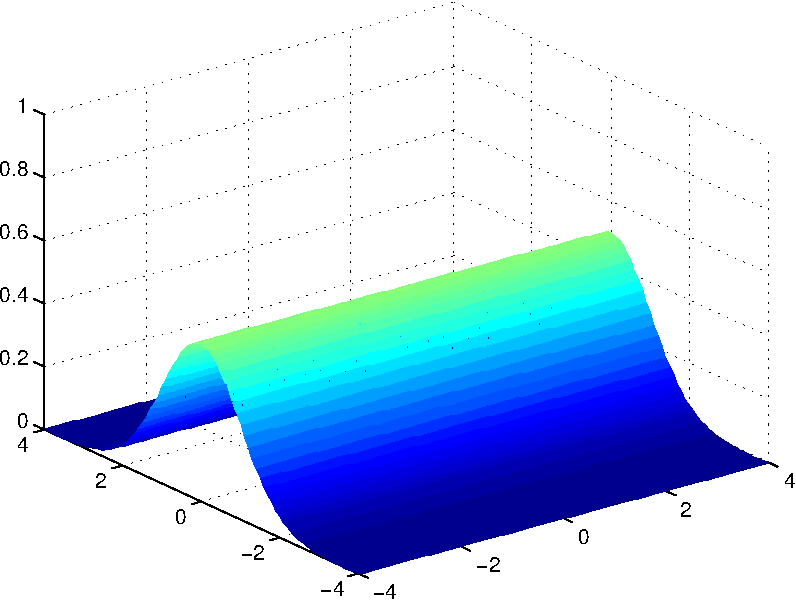
\includegraphics[width=0.2\textwidth]{\additivefigsdir/additive_kernel_sum_p2.pdf} & \hspace{-0.4cm} + \hspace{-0.4cm} & 
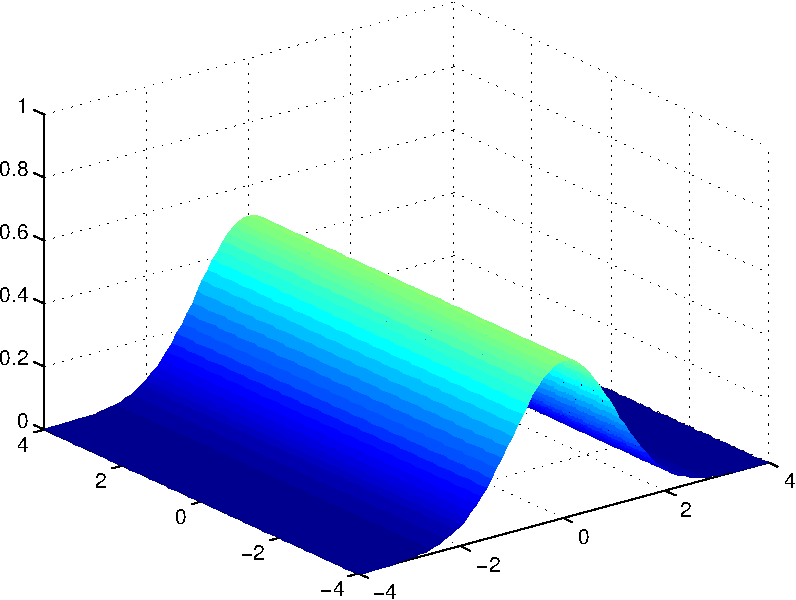
\includegraphics[width=0.2\textwidth]{\additivefigsdir/additive_kernel_sum_p1.pdf} & \hspace{-0.4cm} = \hspace{-0.4cm} & 
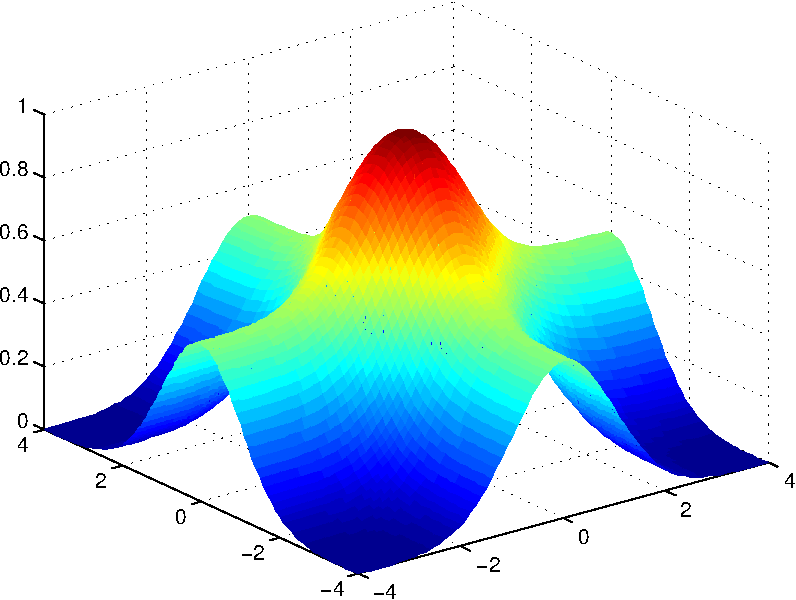
\includegraphics[width=0.2\textwidth]{\additivefigsdir/additive_kernel.pdf} &
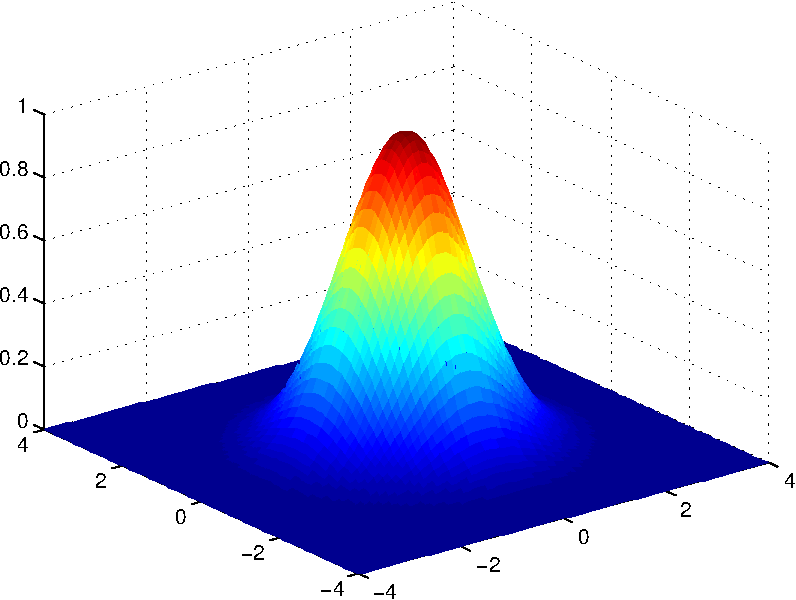
\includegraphics[width=0.2\textwidth]{\additivefigsdir/sqexp_kernel.pdf} \\
$k_1(x_1, x_1')$ & & $k_2(x_2, x_2')$ & & $k_1(x_1,x_1') + k_2(x_2,x_2')$ &$k_1(x_1,x_1')k_2(x_2,x_2')$ \\
1D kernel & & 1D kernel & & 1st order kernel & 2nd order kernel \\ 
%& & & & & \\
%(Second Order) & & & & & Additive Kernel \\
$\downarrow$ & & $\downarrow$ & & $\downarrow$ & $\downarrow$  \\
\hspace{-0.2cm}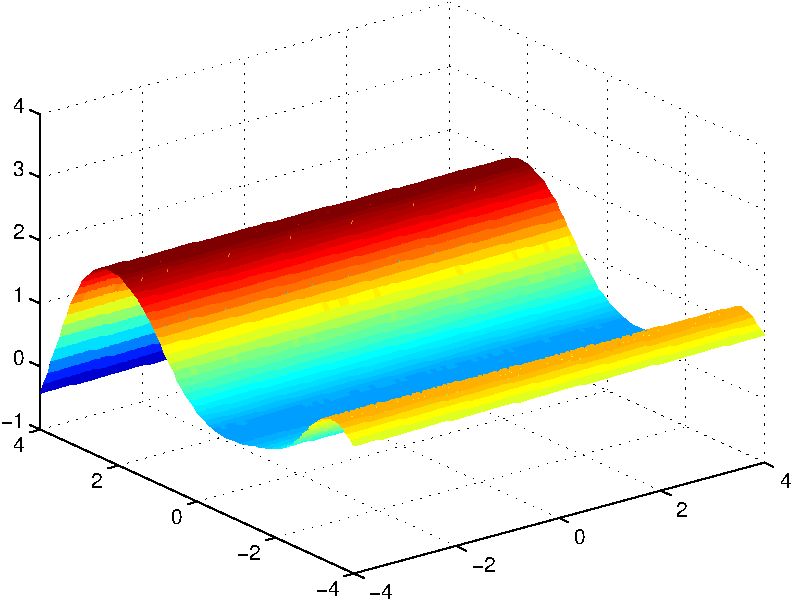
\includegraphics[width=0.2\textwidth]{\additivefigsdir/additive_kernel_draw_sum_p1.pdf}& \hspace{-0.4cm} + \hspace{-0.4cm}& 
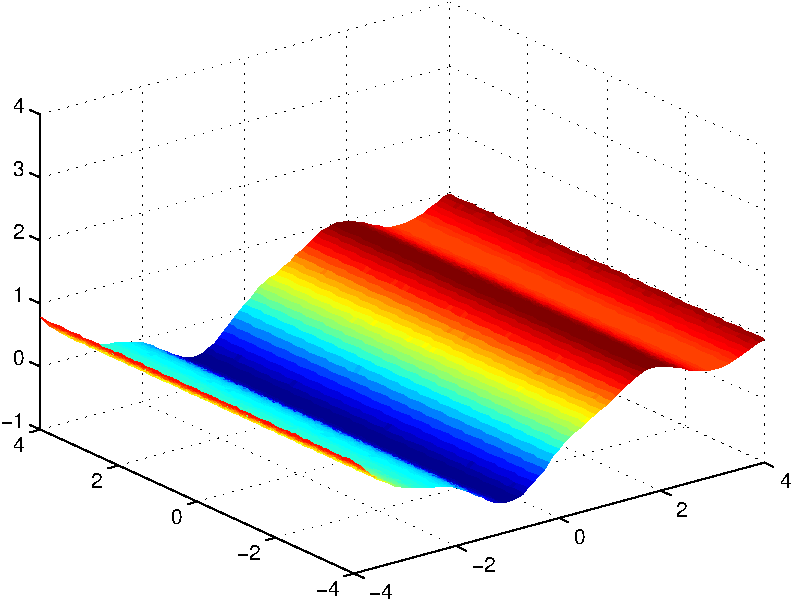
\includegraphics[width=0.2\textwidth]{\additivefigsdir/additive_kernel_draw_sum_p2.pdf}& \hspace{-0.4cm} = \hspace{-0.4cm}&
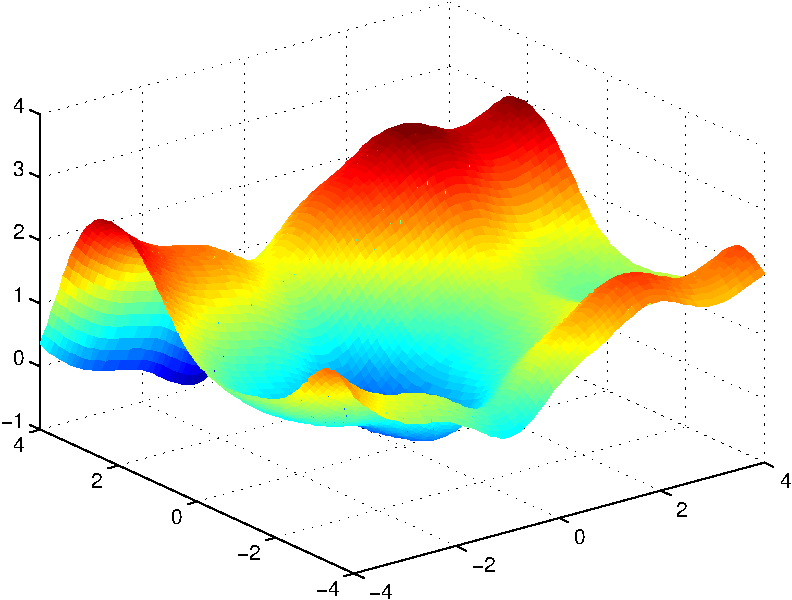
\includegraphics[width=0.2\textwidth]{\additivefigsdir/additive_kernel_draw_sum.pdf} &
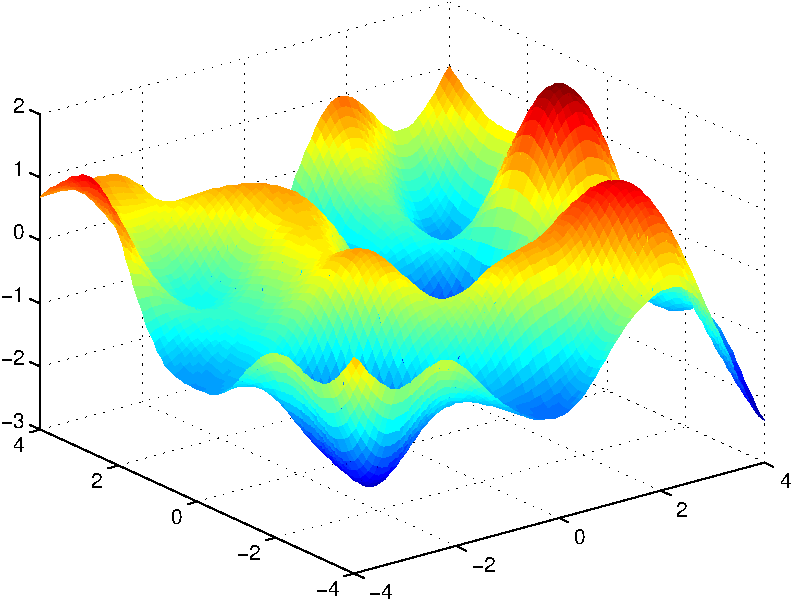
\includegraphics[width=0.2\textwidth]{\additivefigsdir/sqexp_draw.pdf} \\
$f_1(x_1)$ & & $f_2(x_2)$ & & $f_1(x_1) + f_2(x_2)$ & $f(x_1, x_2)$ \\
draw from & & draw from & & draw from & draw from\\
1D GP prior & & 1D GP prior & & 1st order GP prior & 2nd order GP prior\\
%Draw from product kernel GP prior & Draw from additive kernel GP prior\\
\end{tabular}
\caption[Additive kernels correspond to additive functions]{A first-order additive kernel, and a product kernel.  Left: a draw from a first-order additive kernel corresponds to a sum of draws from one-dimensional kernels.  Right: functions drawn from a product kernel prior have weaker long-range dependencies, and less long-range structure.
%In this example, both kernels are composed of one dimensional squared-exponential kernels, but this need not be the case in general.
}
\label{fig:kernels}
\end{figure}

Figure \ref{fig:kernels} compares, for two-dimensional functions, a first-order additive kernel with a second-order kernel. We can see that a GP with a first-order additive kernel is an example of a GAM:  Each function drawn from this model is a sum of orthogonal one-dimensional functions.  Compared to functions drawn from the higher-order GP, draws from the first-order GP have more long-range structure.

  %The only weaknesses with this method are due to over-fitting the kernel hyperparameters, the kernel not being rich enough to capture the structure exhibited by the data, or due to the optimization process not finding the global optima of the hyperparameters.

%\subsection{Additivity in the wild}

We can expect many natural functions to depend only on sums of low-order interactions.  For example, the price of a house or car will presumably be well approximated by a sum of prices of individual features, such as a sun-roof.  
%Other features of the object may depend on the size of the object to jointly determine the price.  
Other parts of the price may depend jointly on a small set of features, such as the size and building materials of a house.
Capturing these regularities will mean that a model can confidently extrapolate to unseen combinations of features.


%\subsection{Additive Covariance}

%Figure \ref{fig:draws} shows that functions drawn from sqexp prior in high dimensions can have tons of zero crossings, and thus will take alot of data to learn.

%\subsection{Why additive functions can be expected to be a good model}

\section{Additive Kernels}
%\subsection{Definition}


We now give a precise definition of additive kernels.  We first assign each dimension $i \in \{1 \dots D\}$ a one-dimensional \emph{base kernel} $k_i(x_i, x'_i)$.  We then define the first order, second order and $n$th order additive kernel as:
\begin{eqnarray}
k_{add_1}({\bf x, x'}) & = & \sigma_1^2 \sum_{i=1}^D k_i(x_i, x_i') \\
k_{add_2}({\bf x, x'}) & = & \sigma_2^2 \sum_{i=1}^D \sum_{j = i + 1}^D k_i(x_i, x_i') k_j(x_j, x_j') \\
k_{add_n}({\bf x, x'}) & = & \sigma_n^2 \sum_{1 \leq i_1 < i_2 < ... < i_n \leq D} \left[ \prod_{d=1}^n k_{i_d}(x_{i_d}, x_{i_d}') \right]
%k_{add_D}({\bf x, x'}) & = & \sigma_D^2 \prod_{d=1}^D k_{d}(x_{d}, x_{d}')
\end{eqnarray}
where $D$ is the dimension of our input space, and $\sigma_n^2$ is the variance assigned to all $n$th order interactions. The $n$th covariance function is a sum of ${D \choose n}$ terms.  In particular, the $D$th order additive covariance function has ${D \choose D} = 1$ term, a product of each dimension's covariance function:
\begin{equation}
k_{add_D}({\bf x, x'}) = \sigma_D^2 \prod_{d=1}^D k_{d}(x_{d}, x_{d}')
\end{equation}
In the case where each base kernel is a one-dimensional squared-exponential kernel, the $D$th-order term corresponds to the multivariate squared-exponential kernel:
\begin{equation}
%\resizebox{\textwidth}{!}{$
k_{add_D}({\bf x, x'}) = \sigma_D^2 \prod_{d=1}^D k_{d}(x_{d}, x_{d}') = \sigma_D^2 \prod_{d=1}^D \exp \Big( -\frac{ ( x_{d} - x_{d}')^2}{2l^2_d} \Big) = \sigma_D^2  \exp \Big( -\sum_{d=1}^D \frac{ ( x_{d} - x_{d}')^2}{2l^2_d} \Big)
%$}
\end{equation}
also commonly known as the Gaussian kernel.  The full additive kernel is a sum of the additive kernels of all orders.
%
\subsection{Parameterization}

The only design choice necessary in specifying an additive kernel is the selection of a one-dimensional base kernel for each input dimension.  Any parameters (such as length-scales) of the base kernels can be learned as usual by maximizing the marginal likelihood of the training data.  

In addition to the hyperparameters of each dimension-wise kernel, additive kernels are equipped with a set of $D$ hyperparameters $\sigma_1^2 \dots \sigma_D^2$ controlling how much variance we assign to each order of interaction.  These ``order variance'' hyperparameters have a useful interpretation:  The $d$th order variance hyperparameter controls how much of the target function's variance comes from interactions of the $d$th order.
%
%% --- Automatically generated by hypers_to_latex.m ---
% Exported at 03-Jun-2011 00:23:44
\begin{table}[h]
\caption{{\small
Hyperparameters for concrete dataset.
}}
\label{tbl:concrete}
\begin{center}
\begin{tabular}{r | r r r r r r r r}
Variable: & cement  & slag  & ash  & water  & plast.  & coarse  & fine  & age  \\ \hline
Sq-exp lengthscale & $3.53$  & $3.90$  & $7.13$  & $1.17$  & $3.94$  & $13.61$  & $2.82$  & $0.54$  \\ 
\hline
Additive lengthscale & $1.42$  & $1.57$  & $3.00$  & $0.08$  & $0.52$  & $298.00$  & $1.46$  & $0.11$  \\
\hline
Order of interaction: & \nth{1} & \nth{2} & \nth{3} & \nth{4} & \nth{5} & \nth{6} & \nth{7} & \nth{8} \\
Additive order variance & $70.6$\% & $13.3$\% & $13.8$\% & $2.3$\% & $0.0$\% & $0.0$\% & $0.0$\% & $0.0$\% \\ \hline
\end{tabular}
\end{center}
\end{table}
% End automatically generated LaTeX

%Table \ref{tbl:concrete} gives an example of hyperparameters learnt by both a SE-GP, and by those learnt by an additive GP whose base kernels are one-dimensional squared exponential kernels.  In this case, the 1st, 2nd and 3rd-order interactions contribute most to the final function.
%
%
Table \ref{tbl:all_orders} shows examples of normalized order variance hyperparameters learned on real datasets.
% --- Automatically generated by hypers_to_latex.m ---
% Exported at 03-Jun-2011 00:22:23
\begin{table}[h]
\caption[Relative variance contribution of each order of the additive model]
{Relative variance contribution of each order in the additive model, on different datasets. Here, the maximum order of interaction is set to 10, or smaller if the input dimension less than 10.  Values are normalized to sum to 100.
}
\label{tbl:all_orders}
\begin{center}
\begin{tabular}{r | r r r r r r r r r r}
Order of interaction & \nth{1} & \nth{2} & \nth{3} & \nth{4} & \nth{5} & \nth{6} & \nth{7} & \nth{8} & \nth{9} & \nth{10} \\ \hline
pima  & $0.1 $ & $0.1 $ & $0.1 $ & $0.3 $ & $1.5 $ & ${\bf 96.4}$ & $1.4 $ & $0.0 $ & & \\
liver  & $0.0 $ & $0.2 $ & ${\bf 99.7 } $ & $0.1 $ & $0.0 $ & $0.0 $ & & & & \\
heart  & ${\bf 77.6} $ & $0.0 $ & $0.0 $ & $0.0 $ & $0.1 $ & $0.1 $ & $0.1 $ & $0.1 $ & $0.1 $ & $22.0 $ \\
concrete  & ${\bf 70.6 } $ & $13.3 $ & $13.8 $ & $2.3 $ & $0.0 $ & $0.0 $ & $0.0 $ & $0.0 $ & & \\
pumadyn-8nh  & $0.0 $ & $0.1 $ & $0.1 $ & $0.1 $ & $0.1 $ & $0.1 $ & $0.1 $ & ${\bf 99.5 } $ & & \\
servo  & ${\bf 58.7 }$ & $27.4 $ & $0.0 $ & $13.9 $ & & & & & & \\
housing  & $0.1 $ & $0.6 $ & ${\bf 80.6 }$ & $1.4 $ & $1.8 $ & $0.8 $ & $0.7 $ & $0.8 $ & $0.6 $ & $12.7 $ \\
\end{tabular}
\end{center}
\end{table}
% End automatically generated LaTeX

On different datasets, the dominant order of interaction estimated by the additive model varies widely.  An additive GP with all of its variance coming from the 1st order is equivalent to a GAM; an additive GP with all its variance coming from the $D$th order is equivalent to a SE-GP.
%
% We can see that the length-scales learnt are not necessarily the same.  This is because, in a normal ARD-style kernel, the length-scale of a dimension is conflated with the variance of the function along that dimension.  The additive kernel separates these two hyperparameters.
%
%This table lets us examine the relative contribution of each order of interaction to the total function variance.  Again, the ARD kernel is equivalent to an additive kernel in which all the variance is constrained to arise only from the highest-order interactions.

%\subsubsection{Model Selection}

Because the hyperparameters can specify which degrees of interaction are important, the additive GP is an extremely general model.  
%By optimizing these hyperparameters, we are approximately performing weighted model selection over a set of $D$ models.
  If the function we are modeling is decomposable into a sum of low-dimensional functions, our model can discover this fact and exploit it (see Figure \ref{fig:synth2d}) .  If this is not the case, the hyperparameters can specify a suitably flexible model.
%In the limit of infinite data, a product kernel and its all-subsets expansion will converge to the same mean function (proof?).  However, in the medium-data regime, the additive kernel can discover structure in the functions it is modeling that the product kernel cannot.

%The expected number of zero crossings is $O(k^d)$ for product kernels (sqexp), $O(kd)$ for first-order additive, and $O\left(k  {d \choose r}\right)$ for $r$th order additive functions. [Conjecture]

%To push the analogy, using a product kernel is analogous to performing polynomial regression when we are forced to use a high-degree polynomial, even when the data do not support it.  One could also view the Gaussian kernel as one which makes the pessimistic assumption that the function we are model can vary independently for each new combination of variables observed.
\subsection{Interpretability}

As noted by \citet{plate1999accuracy}, one of the chief advantages of additive models such as GAM is their interpretability.
% since a high-dimensional function is decomposed into a series of one- or two-dimensional functions.  
Plate also notes that by allowing high-order interactions as well as low-order interactions, one can trade off interpretability with predictive accuracy.  In the case where the hyperparameters indicate that most of the variance in a function can be explained by low-order interactions, it is useful and easy to plot the corresponding low-order functions, as in Figure \ref{fig:interpretable functions}. 

\begin{figure}[h]
\centering
\begin{tabular}{ccc}
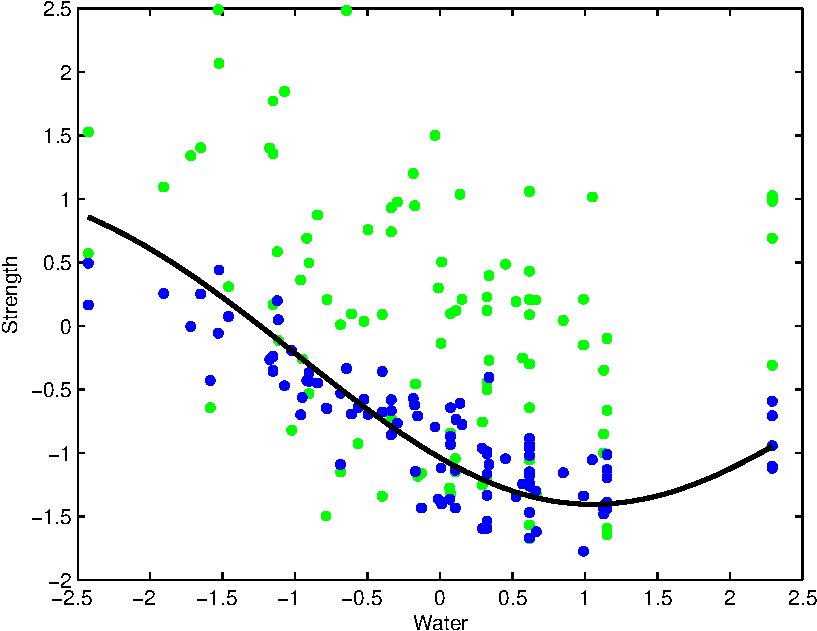
\includegraphics[width=0.3\textwidth]{\additivefigsdir/interpretable_1st_order1.pdf} &
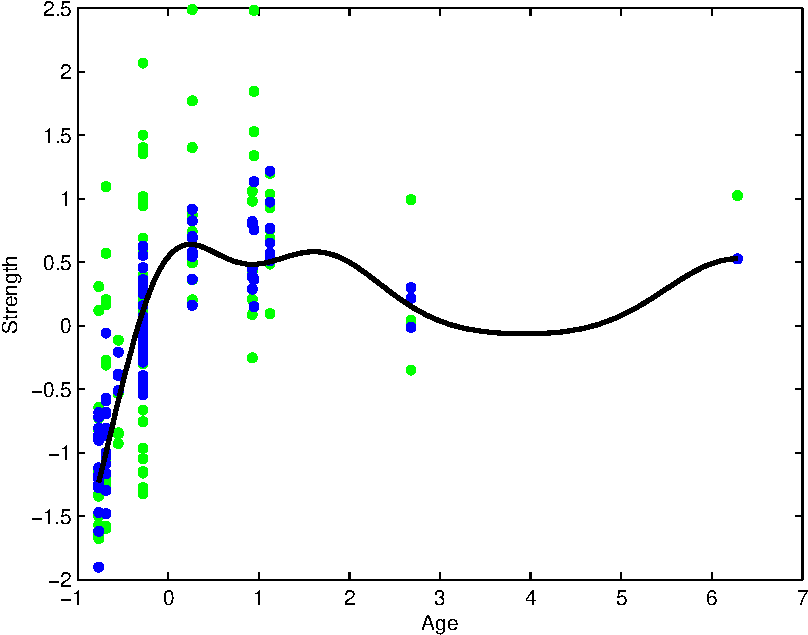
\includegraphics[width=0.3\textwidth]{\additivefigsdir/interpretable_1st_order2.pdf}& 
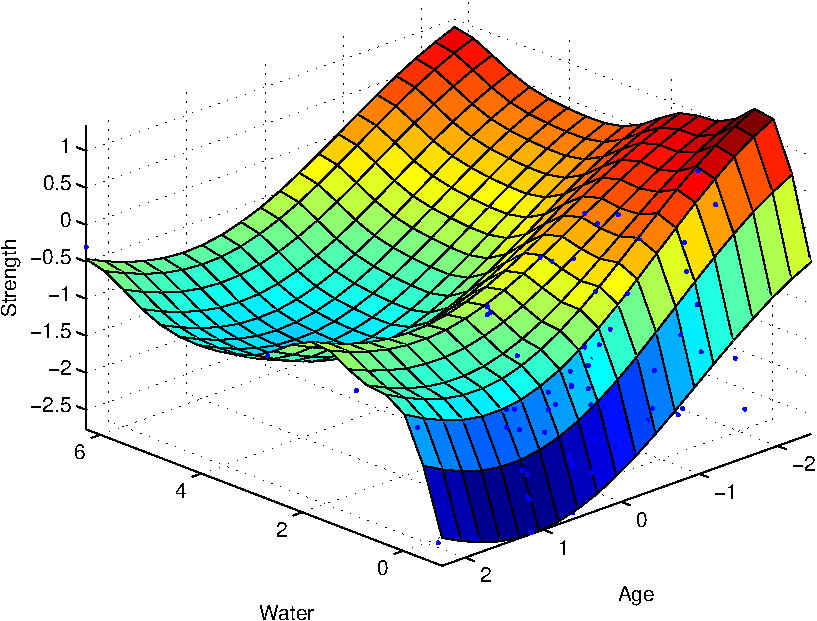
\includegraphics[width=0.3\textwidth]{\additivefigsdir/interpretable_2nd_order1.pdf}\\
\end{tabular}
\caption[Low-order functions describing the concrete dataset]
{Low-order functions on the concrete dataset.  Left, Centre:  By considering only first-order terms of the additive kernel, we recover a form of Generalized Additive Model, and can plot the corresponding 1-dimensional functions.  Green points indicate the original data, blue points are data after the mean contribution from the other dimensions' first-order terms has been subtracted.  The black line is the posterior mean of a GP with only one term in its kernel.  Right:  The posterior mean of a GP with only one second-order term in its kernel.}
\label{fig:interpretable functions}
\end{figure}

%\subsection{Allowable Base Kernels}
%Any one-dimensional base kernel is allowable, and each dimension can use a different base kernel.  One could even specify a mixture of base kernels for each dimension, allowing the hyperparameters to specify the mixture weights.

\subsection{Efficient Evaluation of Additive Kernels}
An additive kernel over $D$ inputs with interactions up to order $n$ has $O(2^n)$ terms.  Na\"{i}vely summing over these terms quickly becomes intractable.  In this section, we show how one can evaluate the sum over all terms in $O(D^2)$.

%\subsection{ Elementary Symmetric Polynomials}
The $n$th order additive kernel corresponds to the $n$th \textit{elementary symmetric polynomial}\cite{macdonald1998symmetric} \cite{stanley2001enumerative}, which we denote $e_n$.  For example:  if $\bf x$ has 4 input dimensions ($D = 4$), and if we let $z_i = k_i(x_i,x_i')$, then
\begin{align*}
%k_{a_1}({\bf x, x'}) & = e_0( z_1, z_2, z_3, z_4 ) & = & 1 \\
k_{add_1}({\bf x, x'}) & = e_1( z_1, z_2, z_3, z_4 ) = z_1 + z_2 + z_3 + z_4 \\
k_{add_2}({\bf x, x'}) & = e_2( z_1, z_2, z_3, z_4 ) = z_1 z_2 + z_1 z_3 + z_1z_4 + z_2 z_3 + z_2 z_4 + z_3 z_4 \\
k_{add_3}({\bf x, x'}) & = e_3( z_1, z_2, z_3, z_4 ) = z_1 z_2 z_3 + z_1 z_2 z_4 + z_1 z_3 z_4 + z_2 z_3 z_4 \\
k_{add_4}({\bf x, x'}) & = e_4( z_1, z_2, z_3, z_4 ) = z_1 z_2 z_3 z_4
\end{align*}
The Newton-Girard formulae give an efficient recursive form for computing these polynomials.  If we define $s_k$ to be the $k$th power sum:  $s_k(z_1,z_2,\dots,z_D) = \sum_{i=1}^Dz_i^k$, then
\begin{equation}
k_{add_n}({\bf x, x'}) = e_n(z_1,\dots,z_D) = \frac{1}{n} \sum_{k=1}^n (-1)^{(k-1)} e_{n-k}(z_1,\dots,z_D)s_k(z_1,\dots,z_D)
\end{equation}
%\begin{equation}
%$s_k(z_1,z_2,\dots,z_n) = z_1^k + z_2^k + \dots + z_D^k = \sum_{i=1}^Dz_i^k$.
%\end{equation}
Where $e_0 \triangleq 1$.  The Newton-Girard formulae have time complexity $O( D^2 )$, while computing a sum over an exponential number of terms.
%\subsection{Evaluation of Derivatives}

Conveniently, we can use the same trick to efficiently compute all of the necessary derivatives of the additive kernel with respect to the base kernels.  We merely need to remove the kernel of interest from each term of the polynomials:
\begin{align}
\frac{\partial k_{add_n}}{\partial z_j} & = e_{n-1}(z_1,\dots,z_{j-1},z_{j+1}, \dots z_D)
% & = \frac{1}{n-1} \sum_{k=1}^{n-1} (-1)^{(k-1)} e_{n-k-1}(z_1,\dots,z_{j-1},z_{j+1}, \dots z_D)s_k(z_1,\dots,z_{j-1},z_{j+1}, \dots z_D)
\end{align}
This trick allows us to optimize the base kernel hyperparameters with respect to the marginal likelihood.

%  The final derivative is a sum of multilinear terms, so if only one term depends on the hyperparameter under consideration, we can factorise it out and compute the sum with one degree less.
\subsection{Computation}
The computational cost of evaluating the Gram matrix of a product kernel (such as the SE kernel) is $O(N^2D)$, while the cost of evaluating the Gram matrix of the additive kernel is $O(N^2DR)$, where R is the maximum degree of interaction allowed (up to D).  In higher dimensions, this can be a significant cost, even relative to the fixed $O(N^3)$ cost of inverting the Gram matrix.
%
However, as our experiments show, typically only the first few orders of interaction are important for modeling a given function; hence if one is computationally limited, one can simply limit the maximum degree of interaction without losing much accuracy.

%\subsection{Code}
Additive Gaussian processes are particularly appealing in practice because their use requires only the specification of the base kernel.  All other aspects of GP inference remain the same.  All of the experiments in this paper were performed using the standard GPML toolbox\footnote{Available at \texttt{http://www.gaussianprocess.org/gpml/code/}}; code to perform all experiments is available at the author's website.\footnote{Example code available at: \texttt{http://mlg.eng.cam.ac.uk/duvenaud/}}


\section{Related Work}

Plate\cite{plate1999accuracy} constructs a form of additive GP, but using only the first-order and $D$th order terms.  This model is motivated by the desire to trade off the interpretability of first-order models, with the flexibility of full-order models.  Our experiments show that often, the intermediate degrees of interaction contribute most of the variance.

A related functional ANOVA GP model\cite{kaufman2010bayesian} decomposes the \emph{mean} function into a weighted sum of GPs. However, the effect of a particular degree of interaction cannot be quantified by that approach. Also, computationally, the Gibbs sampling approach used in \cite{kaufman2010bayesian} is disadvantageous.
%[Todo:  read and mention  and \cite{friedman1981projection} from Hannes]

%\subsection{Multiple Kernel Learning}

%Our current framework relates to Multiple Kernel Learning in that we are learning the weights in a certain mixture of kernels.  
Christoudias et al.\cite{christoudias2009bayesian} previously showed how mixtures of kernels can be learnt by gradient descent in the Gaussian process framework.  They call this \emph{Bayesian localized multiple kernel learning}.
However, their approach learns a mixture over a small, fixed set of kernels, while our method learns a mixture over all possible products of those kernels.

\subsection{Hierarchical Kernel Learning}

\begin{figure}
\centering
\begin{tabular}{c|c|c|c}
\hspace{-0.06in} 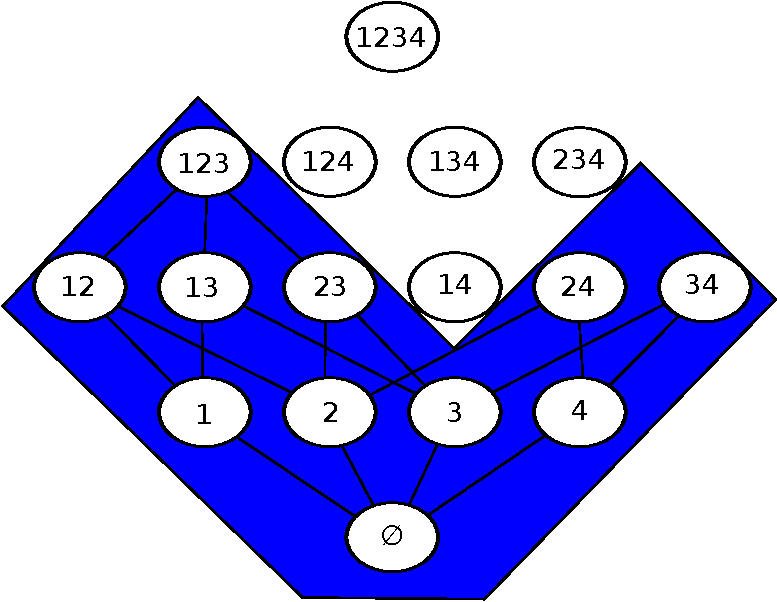
\includegraphics[width=0.23\textwidth]{\additivefigsdir/compare_models/hkl.pdf} \hspace{-0.07in} &
\hspace{-0.06in} 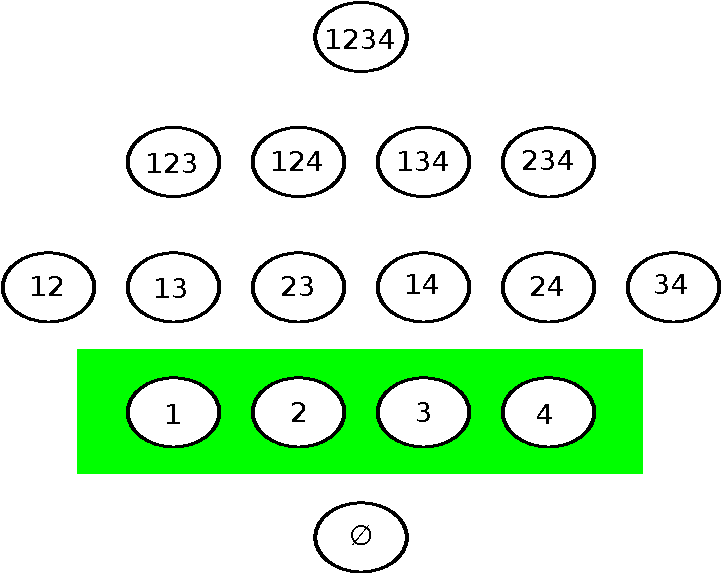
\includegraphics[width=0.23\textwidth]{\additivefigsdir/compare_models/gam.pdf} \hspace{-0.07in} &
\hspace{-0.06in} 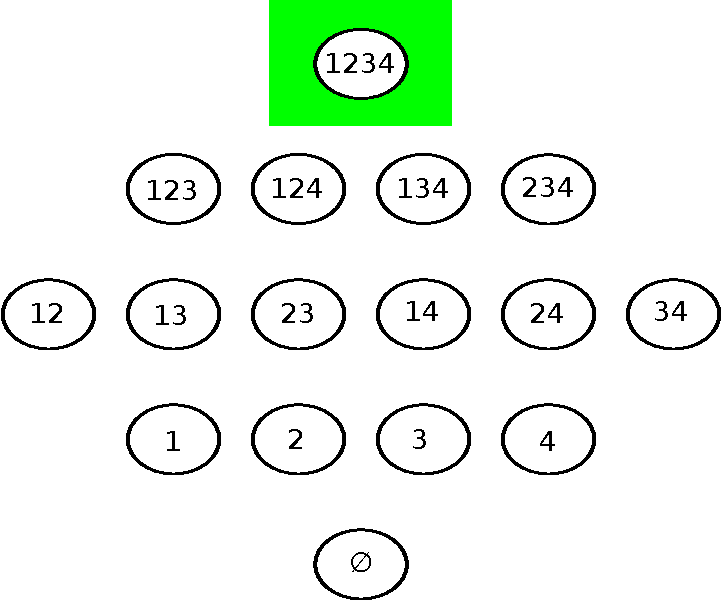
\includegraphics[width=0.23\textwidth]{\additivefigsdir/compare_models/ard.pdf} \hspace{-0.07in} &
\hspace{-0.06in} 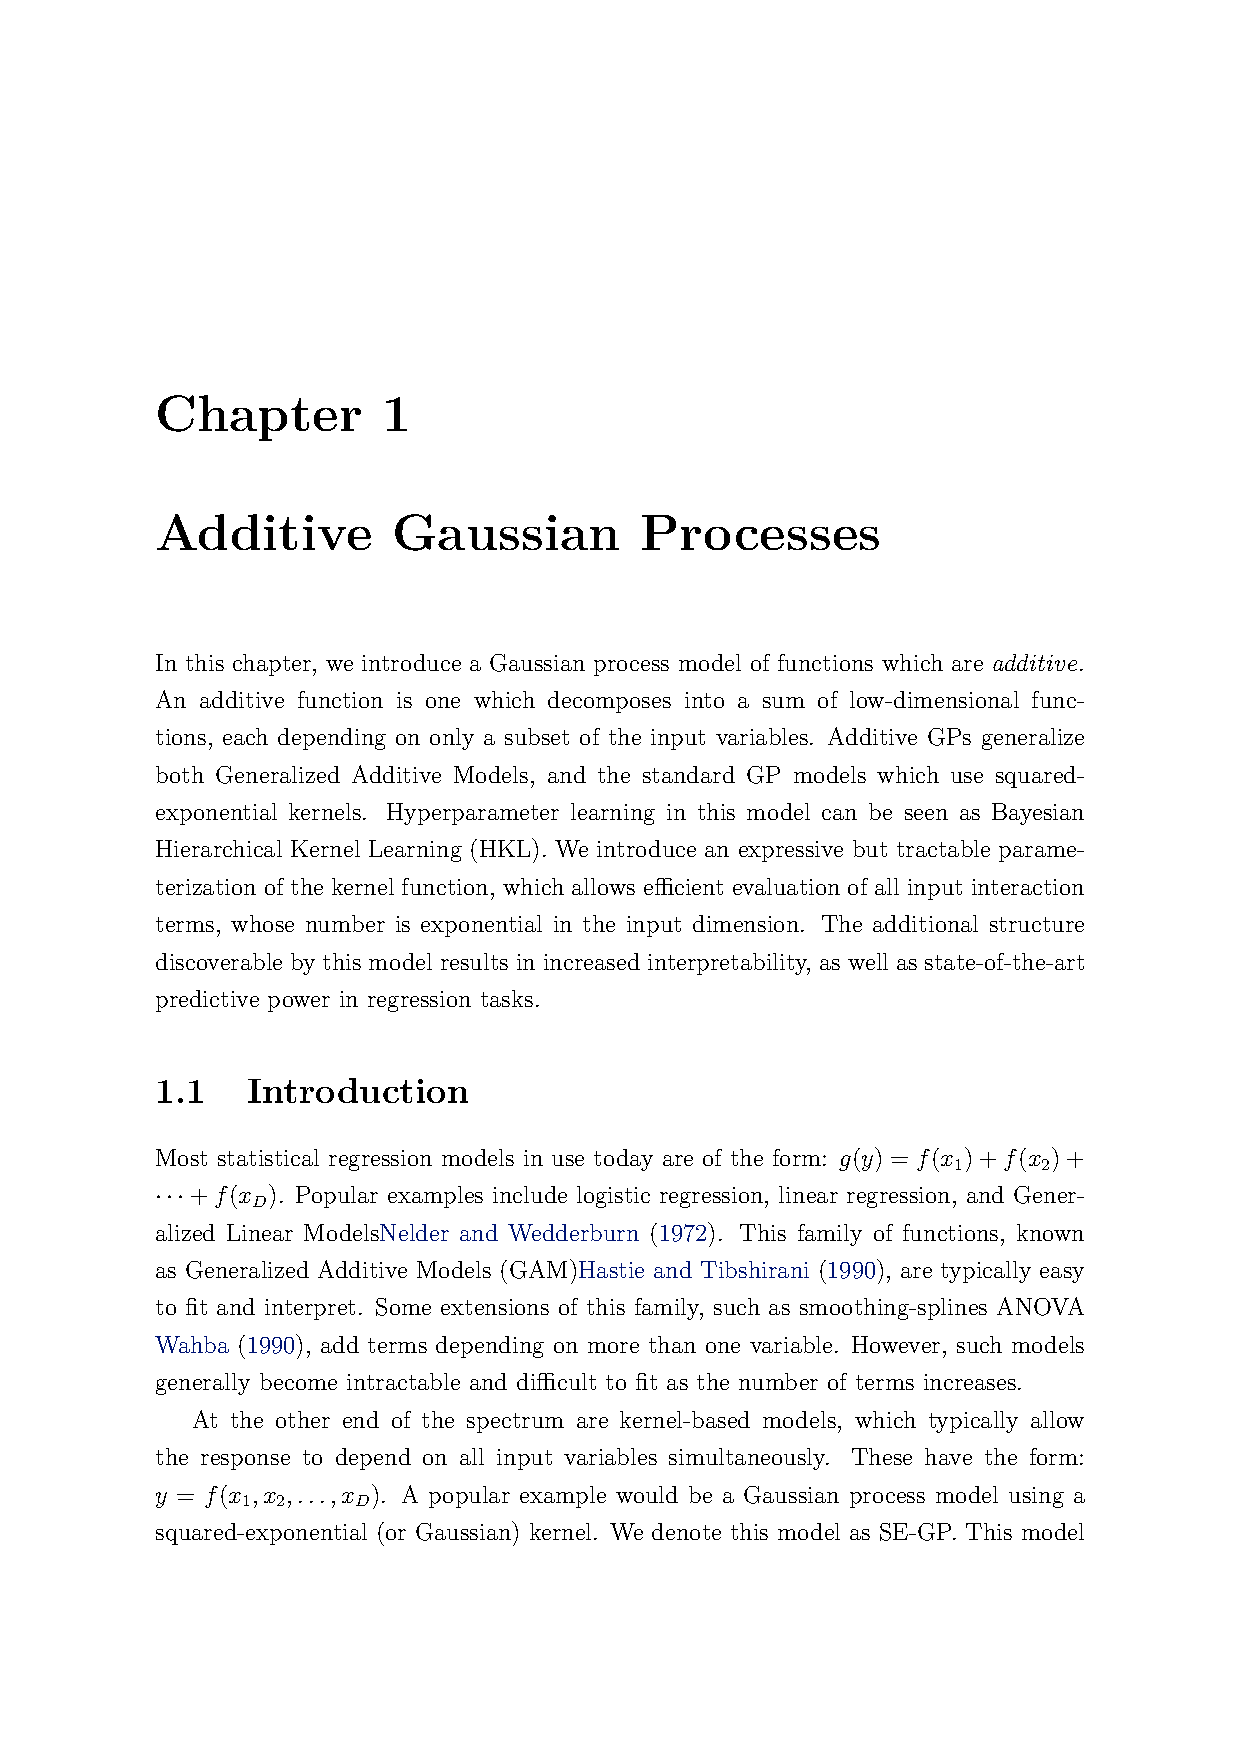
\includegraphics[height=0.19\textwidth]{\additivefigsdir/compare_models/additive.pdf} \\
HKL kernel & GP-GAM kernel & Squared-exp GP & Additive GP kernel\\
 & & kernel & \\
\end{tabular}
\caption[A comparison of different additive model classes]
{
%A comparison of model flexibility between HKL, additive GPs, the GP-Generalized Additive Model, and the squared-exponential GP model.  
A comparison of different additive model classes.  Nodes represent different interaction terms, ranging from first-order to fourth-order interactions.  Far left:  HKL can select a hull of interaction terms, but must use a pre-determined weighting over those terms.  Far right: the additive GP model can weight each order of interaction seperately.  Neither the HKL nor the additive model dominate one another in terms of flexibility, however the GP-GAM and the SE-GP are special cases of additive GPs. }
\label{hulls-figure}
\end{figure}

Bach\cite{DBLP:journals/corr/abs-0909-0844} uses a regularized optimization framework to learn a weighted sum over an exponential number of kernels which can be computed in polynomial time.  The subsets of kernels considered by this method are restricted to be a \textit{hull} of kernels.\footnote{In the setting we are considering in this paper, a hull can be defined as a subset of all terms such that if term $\prod_{j \in J} k_j(\bf x, x')$ is included in the subset, then so are all terms $\prod_{j \in J / i} k_j(\bf x, x')$, for all $i \in J$.  For details, see \cite{DBLP:journals/corr/abs-0909-0844}.}
Given each dimension's kernel, and a pre-defined weighting over all terms, HKL performs model selection by searching over hulls of interaction terms.
% \subsubsection{All-subsets kernel with uniform weightings}
In \cite{DBLP:journals/corr/abs-0909-0844}, Bach also fixes the relative weighting between orders of interaction with a single term $\alpha$, computing the sum over all orders by:
\begin{equation}
\label{eqn:uniform}
k_{a}({\bf x, x'}) = v_D^2 \prod_{d=1}^D \left(1 + \alpha k_{d}(x_{d}, x_{d}') \right)
\end{equation}
which has computational complexity $O(D)$.  However, this formulation forces the weight of all $n$th order terms to be weighted by $\alpha^n$.

Figure \ref{hulls-figure} contrasts the HKL hull-selection method with the Additive GP hyperparameter-learning method. Neither method dominates the other in flexibility.  The main difficulty with the approach of \cite{DBLP:journals/corr/abs-0909-0844} is that hyperparameters are hard to set other than by cross-validation.  In contrast, our method optimizes the hyperparameters of each dimension's base kernel, as well as the relative weighting of each order of interaction. 


\subsection{ANOVA Procedures}

Vapnik \cite{vapnik1998statistical} introduces the support vector ANOVA decomposition, which has the same form as our additive kernel.  However, they recommend approximating the sum over all $D$ orders with only one term ``of appropriate order'', presumably because of the difficulty of setting the hyperparameters of an SVM. Stitson et al.\cite{stitson1999support} performed experiments which favourably compared the support vector ANOVA decomposition to polynomial and spline kernels.  They too allowed only one order to be active, and set hyperparameters by cross-validation.
%
%  The order of the kernel, kernel hyperparameters, the allowable regression error $\epsilon$, and the cost hyperparameter $c$ were all set by a lengthy cross-validation process.

%\subsection{Smoothing Splines ANOVA}
A closely related procedure from the statistics literature is smoothing-splines ANOVA (SS-ANOVA)\cite{wahba1990spline}. An SS-ANOVA model is estimated as a weighted sum of splines along each dimension, plus a sum of splines over all pairs of dimensions, all triplets, etc, with each individual interaction term having a separate weighting parameter.  Because the number of terms to consider grows exponentially in the order, in practice, only terms of first and second order are usually considered.  Learning in SS-ANOVA is usually done via penalized-maximum likelihood with a fixed sparsity hyperparameter.
%\cite{shawe2004kernel} define ANOVA kernels thusly: "The ANOVA kernel of degree d is like the all-subsets kernel except that it is restricted to subsets of the given cardinality $d$."

% estimated by generalized cross-validation\cite{craven1978smoothing}. 
%MARS\cite{friedman1991multivariate} is another spline-based regression method.

In contrast to these procedures, our method can easily include all $D$ orders of interaction, each weighted by a separate hyperparameter. As well, we can learn kernel hyperparameters individually per input dimension, allowing automatic relevance determination to operate.

\subsection{Non-local Interactions}

%In this section we give one motivation for why low-order interactions might help our predictive accuracy.
%
%The SE-GP model relies on local smoothing to make predictions at novel locations.  Recent work by Bengio et. al. discusses the limitations
By far the most popular kernels for regression and classification tasks on continuous data are the squared exponential (Gaussian) kernel, and the Mat\'{e}rn kernels.  These kernels depend only on the scaled Euclidean distance between two points, both having the form: $ k({\bf x, x'}) = f(\sum_{d=1}^D \left( x_{d} - x_{d}' \right)^2 / l_d^2)$.
%\begin{eqnarray}
%k_{se}({\bf x, x'}) & = & v_D^2  \exp \left( -\frac{r^2}{2} \right) \\
%k_{\nu}({\bf x, x'}) & = & \frac{2^{1-\nu}}{\Gamma(\nu)}\left(\sqrt{2\nu}r\right) K_\nu \left(\sqrt{2\nu}r\right)
%\end{eqnarray}
%Where
%\begin{equation}
%$r = \sqrt{\sum_{d=1}^D \left( x_{d} - x_{d}' \right)^2 / l_d^2 }$.
%\end{equation}
Bengio et al.\cite{bengio2006curse} argue that models based on squared-exponential kernels are particularily susceptible to the \textit{curse of dimensionality}.  They emphasize that the locality of the kernels means that these models cannot capture non-local structure.  They argue that many functions that we care about have such structure.  Methods based solely on local kernels will require training examples at all combinations of relevant inputs.

\begin{figure}[h]
\centering
\begin{tabular}{cccc}
\hspace{-0.25in} 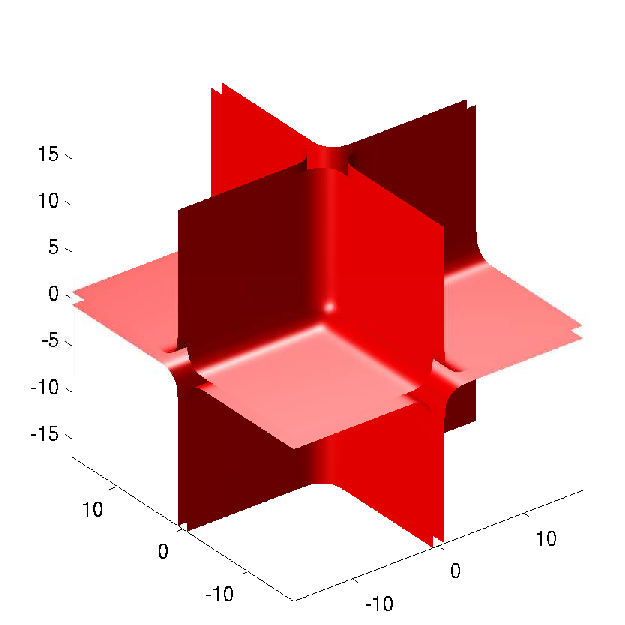
\includegraphics[width=0.27\textwidth]{\additivefigsdir/3d_add_kernel_1.pdf} &
\hspace{-0.25in} 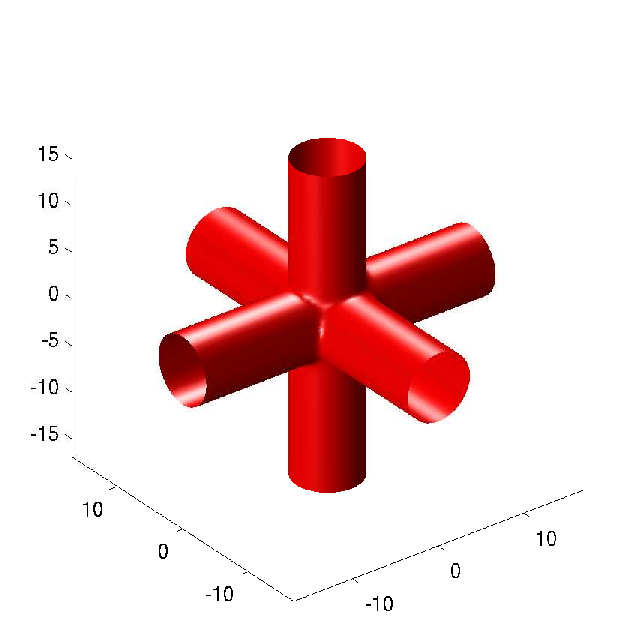
\includegraphics[width=0.27\textwidth]{\additivefigsdir/3d_add_kernel_2.pdf} &
\hspace{-0.25in} 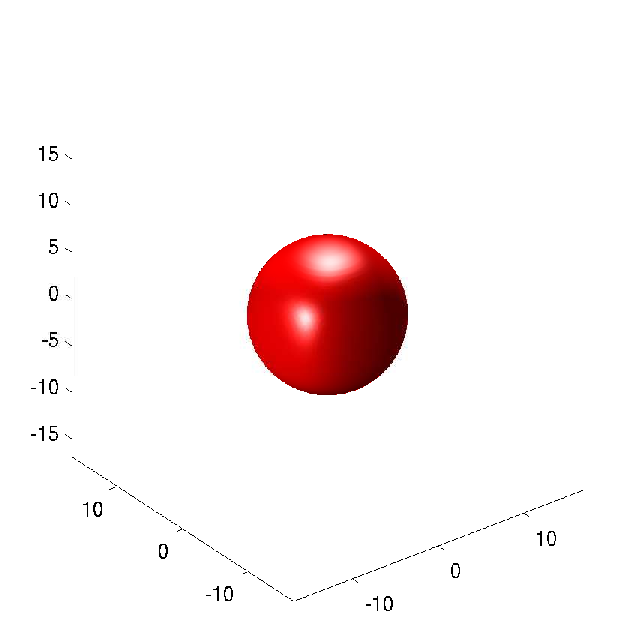
\includegraphics[width=0.27\textwidth]{\additivefigsdir/3d_add_kernel_3.pdf} & 
\hspace{-0.25in} 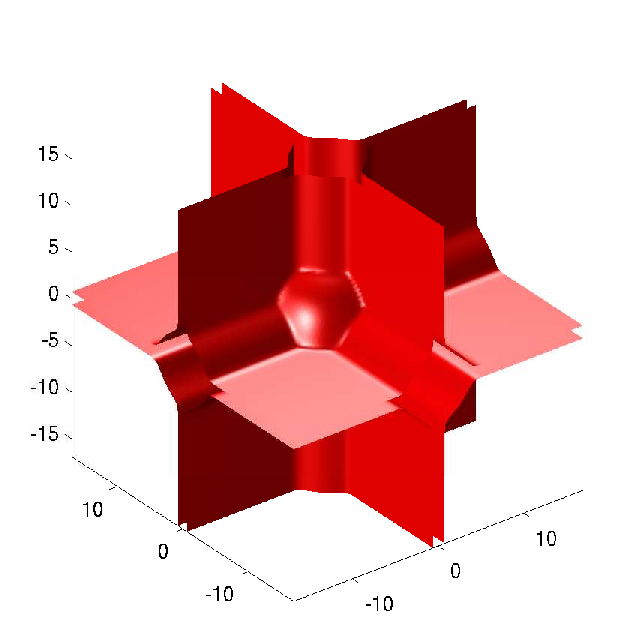
\includegraphics[width=0.27\textwidth]{\additivefigsdir/3d_add_kernel_321.pdf}\\
1st order interactions & 2nd order interactions & 3rd order interactions & All interactions \\
$k_1 + k_2 + k_3$ & $k_1k_2 + k_2k_3 + k_1k_3$ & $k_1k_2k_3$ & \\
& & (Squared-exp kernel) & (Additive kernel)\\
\end{tabular}
\caption[Isocontours of additive kernels in 3 dimensions]
{Isocontours of additive kernels in 3 dimensions.  The third-order kernel only considers nearby points relevant, while the lower-order kernels allow the output to depend on distant points, as long as they share one or more input value.}
\label{fig:kernels3d}
\end{figure}

Additive kernels have a much more complex structure, and allow extrapolation based on distant parts of the input space, without spreading the mass of the kernel over the whole space.  For example, additive kernels of the second order allow strong non-local interactions between any points which are similar in any two input dimensions.
Figure \ref{fig:kernels3d} provides a geometric comparison between squared-exponential kernels and additive kernels in 3 dimensions.


\section{Experiments}



\subsection{Experimental Setup}
%\subsubsection{Learning}

%\subsubsection{Overfitting}
%A multivariate squared exponential kernel has $D + 1$ hyperparameters, while an additive function with one hyperparameter per dimension (e.g., a scale parameter) on each dimension's covariance function will have $D \times 2$ hyperparameters.  Because each additional hyperparameter increases the tendency to overfit, we recommend allowing only one hyperparameter per input dimension. 

%
%Since there always exists a parameterization of the additive function corresponding to the product kernel, we initialize the hyperparameter search for the additive kernel by first learning hyperparameters for the equivalent product kernel.  This ensures that we start our search in a reasonable area of hyperparameter space.
%
%  Results were averaged over 10 cross-validation folds.  To limit the possibility of overfitting, we parametrized each of our one-dimensional kernel functions with only the lengthscale.  
%Note that this parameterization is still more flexible than previous methods (HKL, SS-ANOVA).  % This needs to be double-checked.

%\subsubsection{Initialization}
%We tried 2 different hyperparameterizations, and 3 initialization strategies: \texttt{vo} indicates learning only the variance parameter of each one-dimensional kernel, and \texttt{lo} indicates learning only the lengthscale.  \texttt{grow} indicates that the model was initialized with only 1st-order interactions, and higher interactions were added in stages.  \texttt{ard init} indicates that lengthscales were initialized by first optimizing the hyperparameters of a squared-exp kernel, then copying the lengthscales for use in an additive kernel.
%\subsection{Models}

On a diverse collection of datasets, we compared five different models.  In the results tables below, GP Additive refers to a GP using the additive kernel with squared-exp base kernels.  For speed, we limited the maximum order of interaction in the additive kernels to 10.  GP-GAM denotes an additive GP model with only first-order interactions.  GP Squared-Exp is a GP model with a squared-exponential ARD kernel.  HKL\footnote{Code for HKL available at \texttt{http://www.di.ens.fr/\textasciitilde fbach/hkl/}} was run using the all-subsets kernel, which corresponds to the same set of kernels as considered by the additive GP with a squared-exp base kernel.     

%For all 3 GP models, we allowed 5 multiple restarts for all of our hyperparameter maximization steps, choosing the set of hyperparameters with the highest training-set marginal likelihood.  We ran each hyperparameter search for 500 function evaluations by the usual method of maximizing marginal likelihood, using L-BFGS \cite{nocedal1980updating}.  In addition to kernel hyperparameters, we fit a constant mean function to the data.
For all GP models, we fit hyperparameters by the standard method of maximizing training-set marginal likelihood, using L-BFGS \cite{nocedal1980updating} for 500 iterations, allowing five random restarts.  In addition to learning kernel hyperparameters, we fit a constant mean function to the data.
%
In the classification experiments, GP inference was done using Expectation Propagation \cite{minka2001expectation}.

\subsection{Bach Synthetic Dataset}
In addition to standard UCI repository datasets, we generated a synthetic dataset following the same recipe as \cite{DBLP:journals/corr/abs-0909-0844}: From a covariance matrix drawn from a Wishart distribution with 1024 degrees of freedom, we select 8 variables.  We then construct the non-linear function $f(X) = \sum_{i=1}^4 \sum_{j=1+1}^4 X_i X_j + \epsilon$, which sums all 2-way products of the first 4 variables, and adds Gaussian noise $\epsilon$.  This dataset is one which can be predicted well by a kernel which is a sum of two-way interactions over the first 4 variables, ignoring the extra 4 noisy copies.

This dataset was designed by \cite{DBLP:journals/corr/abs-0909-0844} to demonstrate the advantages of HKL over GP-ARD. 

 If the dataset is large enough, HKL can construct a hull around only those subsets of cross terms that are optimal for predicting the output.  GP-ARD, in contrast, can only learn to ignore the noisy copy variables, but cannot learn to ignore the higher-term interactions between the predictive variables.  However, a GP with an additive kernel can learn both to ignore irrelevant variables, and to ignore certain orders of interaction.  In this example, the additive GP is able to recover the relevant structure.

%% --- Automatically generated by hypers_to_latex.m ---
% Exported at 29-Apr-2011 15:03:44
\begin{table}[h!]
\caption{{\small
Hyperparameters for bach synth c 200 dataset
}}
\label{tbl:bach synth c 200}
\begin{center}
\begin{tabular}{l | r r r r r r r r}
Variable: & $x_1$  & $x_2$  & $x_3$  & $x_4$  & $x_5$  & $x_6$  & $x_7$  & $x_8$  \\ \hline
ARD Lengthscale & $1.09$  & $0.32$  & $0.09$  & $0.74$  & $760.60$  & $522.32$  & $667.74$  & $886.37$  \\ \hline
ADD Lengthscale & $0.93$  & $0.83$  & $0.04$  & $0.62$  & $473.04$  & $325.51$  & $415.76$  & $551.96$  \\
ADD Variance & $15.48$ & $21.02$ & $0.01$ & $60.93$ & $0.67$ & $0.67$ & $0.67$ & $0.67$ \\ \hline
Order of Interaction: & $1$  & $2$  & $3$  & $4$  & $5$  & $6$  & $7$  & $8$  \\
ADD Order Variance & $0.0$\% & $0.0$\% & $0.0$\% & $0.0$\% & $0.0$\% & $49.0$\% & $0.1$\% & $50.8$\% \\ \hline
\end{tabular}
\end{center}
\end{table}
% End automatically generated LaTeX


%Table \ref{tbl:bach synth c 200} shows the hyperparameters learnt.  Note that while GP-ARD increases the lengthscale of the irrelevant variables, GP-AS reduces the signal variance.
 
\subsection{Results}

Tables \ref{tbl:Regression Mean Squared Error}, \ref{tbl:Regression Negative Log Likelihood}, \ref{tbl:Classification Percent Error} and \ref{tbl:Classification Negative Log Likelihood} show mean performance across 10 train-test splits.  Because HKL does not specify a noise model, it could not be included in the likelihood comparisons.

% --- Automatically generated by resultsToLatex2.m ---
% Exported at 19-Jan-2012 10:55:19
\begin{table}[h]
\caption[Comparison of predictive error on regression problems]
{Regression Mean Squared Error}
\label{tbl:Regression Mean Squared Error}
\begin{center}
\begin{tabular}{l | r r r r r}
Method & \rotatebox{0}{ bach  }  & \rotatebox{0}{ concrete  }  & \rotatebox{0}{ pumadyn-8nh }  & \rotatebox{0}{ servo }  & \rotatebox{0}{ housing }  \\ \hline
Linear Regression & $1.031$ & $0.404$ & $0.641$ & $0.523$ & $0.289$ \\
GP GAM & $1.259$ & $0.149$ & $0.598$ & $0.281$ & $0.161$ \\
HKL & $\mathbf{0.199}$ & $0.147$ & $0.346$ & $0.199$ & $0.151$ \\
GP Squared-exp & $\mathbf{0.045}$ & $0.157$ & $\mathbf{0.317}$ & $\mathbf{0.126}$ & $\mathbf{0.092}$ \\
GP Additive & $\mathbf{0.045}$ & $\mathbf{0.089}$ & $\mathbf{0.316}$ & $\mathbf{0.110}$ & $\mathbf{0.102}$ \\
\end{tabular}
\end{center}
\end{table}
% End automatically generated LaTeX
%
% --- Automatically generated by resultsToLatex2.m ---
% Exported at 19-Jan-2012 10:55:19
\begin{table}[h]
\caption[Comparison of predictive likelihood on regression problems]
{Regression Negative Log Likelihood}
\label{tbl:Regression Negative Log Likelihood}
\begin{center}
\begin{tabular}{l | r r r r r}
Method & \rotatebox{0}{ bach  }  & \rotatebox{0}{ concrete  }  & \rotatebox{0}{ pumadyn-8nh }  & \rotatebox{0}{ servo }  & \rotatebox{0}{ housing }  \\ \hline
Linear Regression & $2.430$ & $1.403$ & $1.881$ & $1.678$ & $1.052$ \\
GP GAM & $1.708$ & $0.467$ & $1.195$ & $0.800$ & $0.457$ \\
GP Squared-exp & $\mathbf{-0.131}$ & $0.398$ & $\mathbf{0.843}$ & $0.429$ & $\mathbf{0.207}$ \\
GP Additive & $\mathbf{-0.131}$ & $\mathbf{0.114}$ & $\mathbf{0.841}$ & $\mathbf{0.309}$ & $\mathbf{0.194}$ \\
\end{tabular}
\end{center}
\end{table}
% End automatically generated LaTeX
%
% --- Automatically generated by resultsToLatex2.m ---
% Exported at 03-Jun-2011 00:23:25
\begin{table}[h]
\caption[Comparison of predictive error on classification problems]
{Classification percent error}
\label{tbl:Classification Percent Error}
\begin{center}
\begin{tabular}{l | r r r r r r}
Method & \rotatebox{0}{ breast }  & \rotatebox{0}{ pima }  & \rotatebox{0}{ sonar }  & \rotatebox{0}{ ionosphere }  & \rotatebox{0}{ liver }  & \rotatebox{0}{ heart }  \\ \hline
Logistic Regression & $7.611$ & $24.392$ & $26.786$ & $16.810$ & $45.060$ & $\mathbf{16.082}$ \\
GP GAM & $\mathbf{5.189}$ & $\mathbf{22.419}$ & $\mathbf{15.786}$ & $\mathbf{8.524}$ & $\mathbf{29.842}$ & $\mathbf{16.839}$ \\
HKL & $\mathbf{5.377}$ & $24.261$ & $\mathbf{21.000}$ & $9.119$ & $\mathbf{27.270}$ & $\mathbf{18.975}$ \\
GP Squared-exp & $\mathbf{4.734}$ & $\mathbf{23.722}$ & $\mathbf{16.357}$ & $\mathbf{6.833}$ & $\mathbf{31.237}$ & $\mathbf{20.642}$ \\
GP Additive & $\mathbf{5.566}$ & $\mathbf{23.076}$ & $\mathbf{15.714}$ & $\mathbf{7.976}$ & $\mathbf{30.060}$ & $\mathbf{18.496}$ \\
\end{tabular}
\end{center}
\end{table}
% End automatically generated LaTeX


% --- Automatically generated by resultsToLatex2.m ---
% Exported at 03-Jun-2011 00:23:28
\begin{table}[h]
\caption[Comparison of predictive likelihood on classification problems]
{Classification negative log-likelihood}
\label{tbl:Classification Negative Log Likelihood}
\begin{center}
\begin{tabular}{l | r r r r r r}
Method & \rotatebox{0}{ breast }  & \rotatebox{0}{ pima }  & \rotatebox{0}{ sonar }  & \rotatebox{0}{ ionosphere }  & \rotatebox{0}{ liver }  & \rotatebox{0}{ heart }  \\ \hline
Logistic Regression & $0.247$ & $0.560$ & $4.609$ & $0.878$ & $0.864$ & $0.575$ \\
GP GAM & $\mathbf{0.163}$ & $\mathbf{0.461}$ & $\mathbf{0.377}$ & $\mathbf{0.312}$ & $\mathbf{0.569}$ & $\mathbf{0.393}$ \\
GP Squared-exp & $\mathbf{0.146}$ & $0.478$ & $\mathbf{0.425}$ & $\mathbf{0.236}$ & $\mathbf{0.601}$ & $0.480$ \\
GP Additive & $\mathbf{0.150}$ & $\mathbf{0.466}$ & $\mathbf{0.409}$ & $\mathbf{0.295}$ & $\mathbf{0.588}$ & $\mathbf{0.415}$ \\
\end{tabular}
\end{center}
\end{table}
% End automatically generated LaTeX


The model with best performance on each dataset is in bold, along with all other models that were not significantly different under a paired t-test. The additive model never performs significantly worse than any other model, and sometimes performs significantly better than all other models.  The difference between all methods is larger in the case of regression experiments. The performance of HKL is consistent with the results in \cite{DBLP:journals/corr/abs-0909-0844}, performing competitively but slightly worse than SE-GP.%  This is especially clear in the case of the regression tasks.

The additive GP performed best on datasets well-explained by low orders of interaction, and approximately as well as the SE-GP model on datasets which were well explained by high orders of interaction (see table \ref{tbl:all_orders}).
Because the additive GP is a superset of both the GP-GAM model and the SE-GP model, instances where the additive GP performs slightly worse are presumably due to over-fitting, or due to the hyperparameter optimization becoming stuck in a local maximum. % Absence of over-fitting may explain the relatively strong performance of GP-GAM on classification tasks.  
Additive GP performance can be expected to benefit from integrating out the kernel hyperparameters.



\subsection{Future Work}
Since the non-local structure capturable by additive kernels is necessarily axis-aligned, we can naturally consider that combining the hyperparameter optimization with an initial rotation of the input space might allow us to recover non-axis aligned additivity in functions.

Note that we are free to choose a different covariance function along each dimension.


\section{Conclusion}

%We present a simple model which generalizes two widely-used classes of models.  A large increase in modeling power is gained at only modest computational cost.
We present additive Gaussian processes: a simple family of models which generalizes two widely-used classes of models.  Additive GPs also introduce a tractable new type of structure into the GP framework.   Our experiments indicate that such additive structure is present in real datasets, allowing our model to perform better than standard GP models.  In the case where no such structure exists, our model can recover arbitrarily flexible models, as well.

In addition to improving modeling efficacy, the additive GP also improves model interpretability:  the order variance hyperparameters indicate which sorts of structure are present in our model.

Compared to HKL, which is the only other tractable procedure able to capture the same types of structure, our method benefits from being able to learn individual kernel hyperparameters, as well as the weightings of different orders of interaction.  Our experiments show that additive GPs are a state-of-the-art regression model.



\outbpdocument{
\bibliographystyle{plainnat}
\bibliography{references.bib}
}





%\begin{figure}
%\centering
%\begin{tabular}{cc}
%\hspace{-0.1in}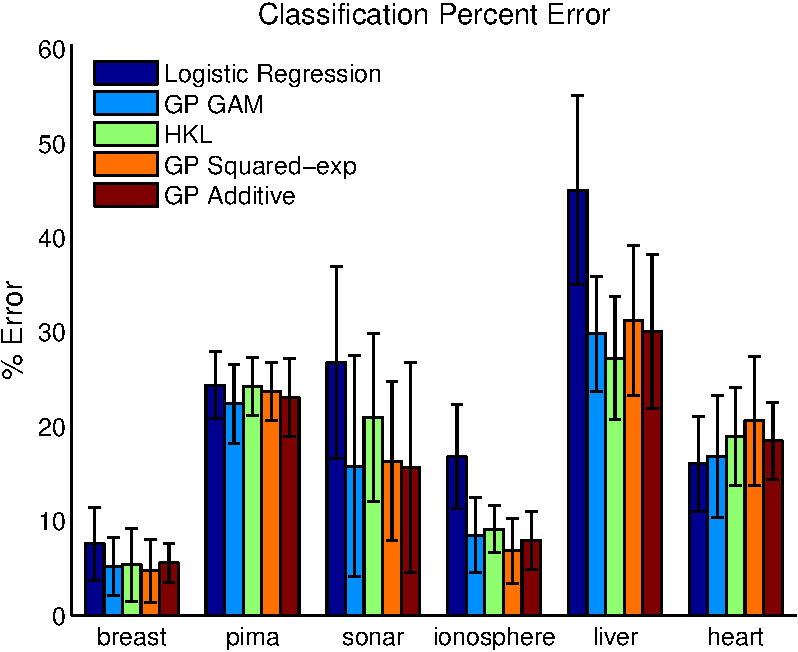
\includegraphics[width=0.475\textwidth]{\additivefigsdir/class_graph.pdf} &
%\hspace{-0.1in}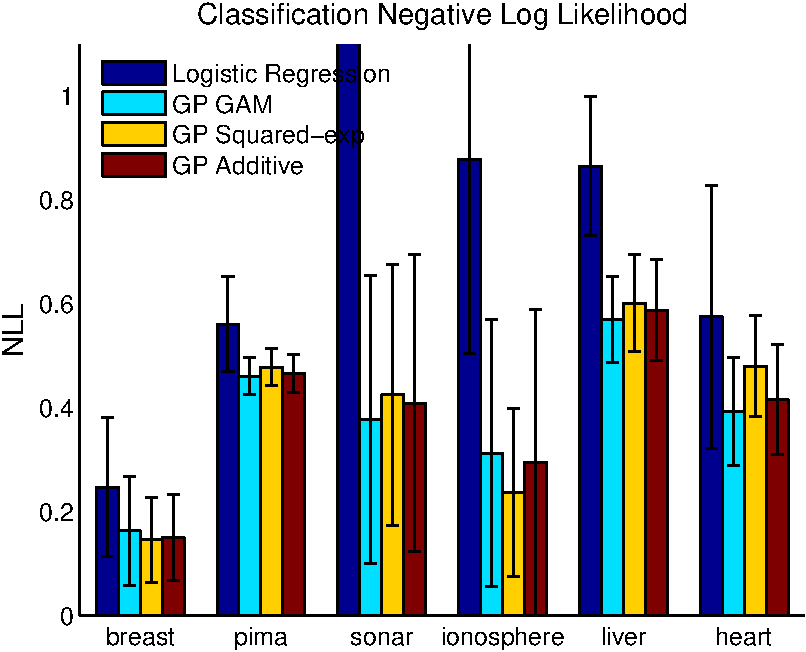
\includegraphics[width=0.475\textwidth]{\additivefigsdir/class_graph_ll.pdf}\\
%\hspace{-0.1in}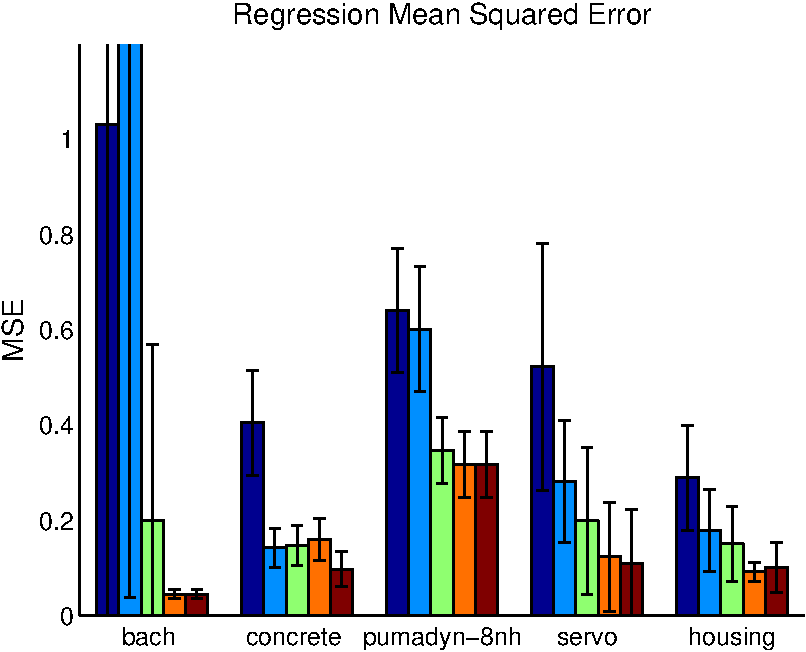
\includegraphics[width=0.475\textwidth]{\additivefigsdir/reg_graph.pdf}& 
%\hspace{-0.1in}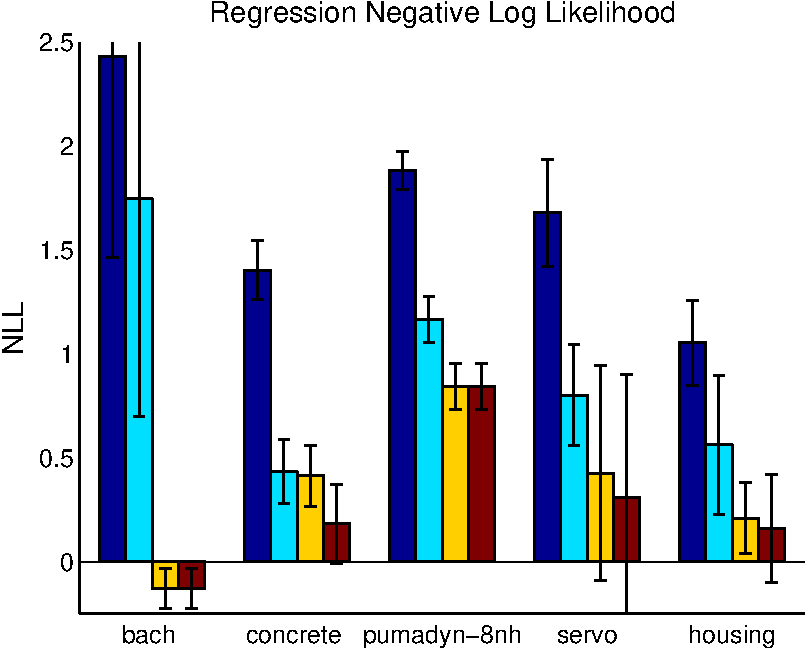
\includegraphics[width=0.475\textwidth]{\additivefigsdir/reg_graph_ll.pdf}\\ 
%\end{tabular}
%\label{fig:results}
%\end{figure}


%\section{Discussion}
%% --- Automatically generated by hypers_to_latex.m ---
% Exported at 12-May-2011 16:56:21
\begin{table}[h]
\caption{{\small
Hyperparameters for housing dataset
}}
\label{tbl:housing}
\begin{center}
\begin{tabular}{l | r r r r r r r r r r r r r}
Variable: & $x_1$  & $x_2$  & $x_3$  & $x_4$  & $x_5$  & $x_6$  & $x_7$  & $x_8$  & $x_9$  & $x_10$  & $x_11$  & $x_12$  & $x_13$  \\ \hline
ARD Lengthscale & $1508.26$  & $504.64$  & $296.62$  & $3.91$  & $0.08$  & $2.21$  & $5.77$  & $2.77$  & $424.77$  & $0.74$  & $233.78$  & $605.23$  & $3.75$  \\ 
\hline
ADD Lengthscale & $392.41$  & $147.62$  & $183.48$  & $12.16$  & $0.04$  & $2.33$  & $5.71$  & $0.49$  & $402.78$  & $0.68$  & $322.01$  & $1027.36$  & $1.48$  \\
ADD Variance & $0.29$ & $0.29$ & $0.29$ & $0.44$ & $0.02$ & $19.14$ & $0.25$ & $0.97$ & $0.29$ & $10.77$ & $0.29$ & $0.29$ & $0.37$ \\ \hline
Order of Interaction: & \nth{1} & \nth{2} & \nth{3} & \nth{4} & \nth{5} & \nth{6} & \nth{7} & \nth{8} & \nth{9} & \nth{10} \\
ADD Order Variance & $0.1$\% & $0.1$\% & $0.1$\% & $0.0$\% & $0.0$\% & $0.0$\% & $0.0$\% & $0.0$\% & $0.0$\% & $99.8$\% \\ \hline
\end{tabular}
\end{center}
\end{table}
% End automatically generated LaTeX

%% --- Automatically generated by hypers_to_latex.m ---
% Exported at 12-May-2011 16:56:20
\begin{table}[h]
\caption{{\small
Hyperparameters for pima dataset
}}
\label{tbl:pima}
\begin{center}
\begin{tabular}{l | r r r r r r r r}
Variable: & $x_1$  & $x_2$  & $x_3$  & $x_4$  & $x_5$  & $x_6$  & $x_7$  & $x_8$  \\ \hline
ARD Lengthscale & $0.30$  & $0.05$  & $4.15$  & $3.62$  & $0.26$  & $1.78$  & $326.52$  & $0.76$  \\ 
\hline
ADD Lengthscale & $0.23$  & $0.05$  & $3.75$  & $6.37$  & $0.27$  & $1.81$  & $107.98$  & $0.58$  \\
ADD Variance & $2.47$ & $0.03$ & $0.86$ & $0.75$ & $0.35$ & $1.56$ & $0.71$ & $60.36$ \\ \hline
Order of Interaction: & \nth{1} & \nth{2} & \nth{3} & \nth{4} & \nth{5} & \nth{6} & \nth{7} & \nth{8} \\
ADD Order Variance & $0.0$\% & $0.1$\% & $0.1$\% & $0.3$\% & $0.0$\% & $29.0$\% & $0.1$\% & $70.4$\% \\ \hline
\end{tabular}
\end{center}
\end{table}
% End automatically generated LaTeX



%As a special case, additive kernels with only one degree of interaction can be computed in something like linear time [cite Yunus?]
 % E = elsympol(Kd(:,:,[1:j-1,j+1:D]),max(R)-1);



 
 
%\subsection{Polynomial Kernels}

%A simple variation on the all-subsets kernel would be one which includes repeated terms, of the form
%\begin{equation}
%k_{h_n}({\bf x, x'}) = v_n^2 \sum_{i_1, \dots, i_n} \prod_{d=1}^n k_{i_d}(x_{i_d}, x_{i_d}') = v_n^2 \prod_{d=1}^n \sum_{i_1, \dots, i_n}^n k_{i_d}(x_{i_d}, x_{i_d}')
%\end{equation}
%This formulation allows repeated terms, such as $x_i^2$ and is equivalent to the polynomial kernel\cite{shawe2004kernel}.  However, this formulation cases the length scale of each dimension to vary with the order of interaction considered.




%[Equation for derivatives]





%The fact that our model is additive does not mean that it ignores multiplicative, or higher-order interactions

